\documentclass[12pt]{article}
\usepackage[spanish]{babel}
\usepackage[utf8]{inputenc}
\usepackage{apacite}
\usepackage{graphicx}
\usepackage{float}
\usepackage{url}
\usepackage{caption}
\usepackage{subcaption}
\graphicspath{{./images/} }
\providecommand{\keywords}[1]{\textbf{\textit{Palabras clave---}} #1}

\title{Análisis de la Nsp15 del SARS-COV2: una aproximación bioinformática en la lucha contra la COVID-19}
\author{Juan Manuel Ruiz Robles}


\begin{document}


\maketitle
\begin{figure}[H]
\centering

\includegraphics[ scale=0.5]{logo}
\end{figure}
\newpage
\tableofcontents
\newpage

\section{Análisis genético}

En primer lugar y como complemento al trabajo, he decidido aportar mi toque personal con un breve análisis bioinformática de la secuencia del SARS-COV2. En NCBI descargué la secuencia completa del virus en formato FASTA, típicamente utilizado en el ámbito científico.
\begin{figure}[H]
\centering
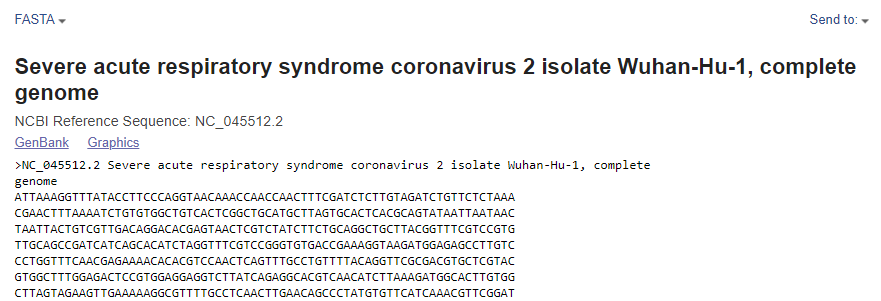
\includegraphics[trim={0 0 0 1.5cm},clip, scale=0.6]{Screenshot_1}
\end{figure}
Esto lo hice porque tengo varias funciones desarrolladas en el ordenador para el lenguaje de programación Python, las cuales me permiten detectar ciertas características de las secuencias genéticas, lo que en este caso, debido a la relevancia de la biología funcional en el estudio del SARS-COV2 tiene cabida en este trabajo.
\newline

Todas las funciones utilizadas son de elaboración propia, realizadas a partir de autoaprendizaje visitando videotutoriales y páginas web. Dichas funciones tratan de imitar los procesos bioquímicos básicos de la célula.
\newline

En general, mi forma de trabajo consiste en tomar la/las secuencias e introducirlas en un archivo FASTA, y tengo una función que me crea una estructura de diccionario en Python, donde el nombre de la secuencia es la clave del diccionario y la secuencia es el “value” o elemento correspondiente a la clave.
\begin{figure}[H]
\raggedright
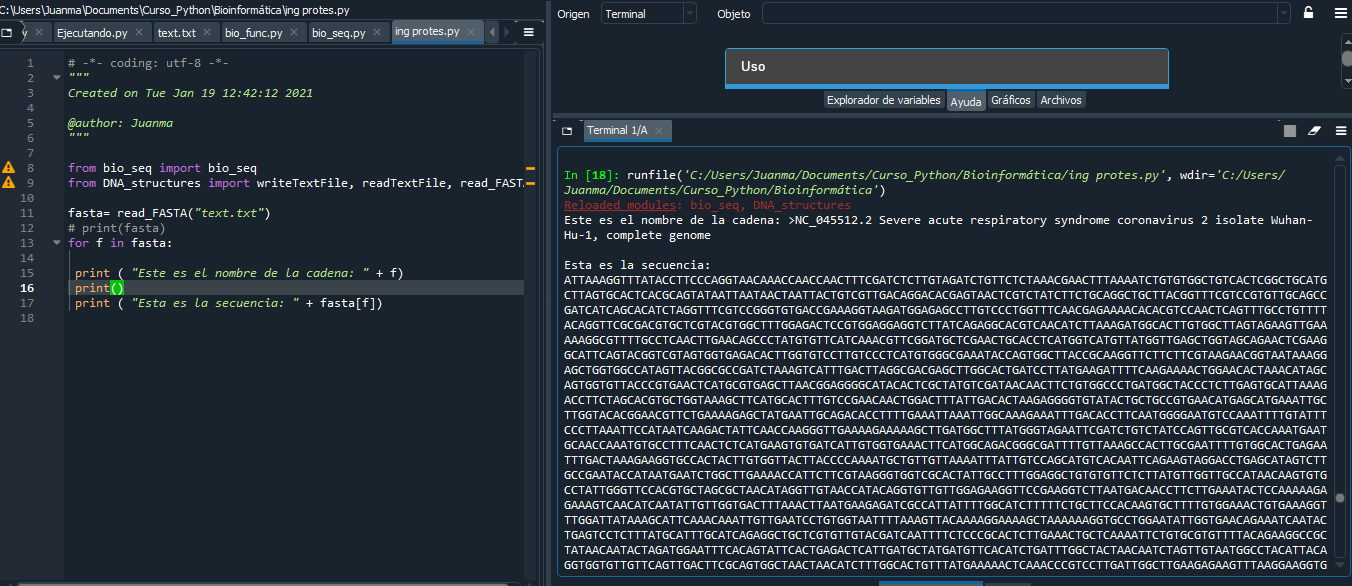
\includegraphics[trim={0 0 0 1.2cm},clip,scale=0.4]{Screenshot_2}
\end{figure}
De esta forma, podemos tener toda secuencia identificada mientras estudiamos diversas características de la misma.
\newline

Por ejemplo, podemos observar la longitud de la secuencia:
\newline
\begin{figure}[H]
\raggedright
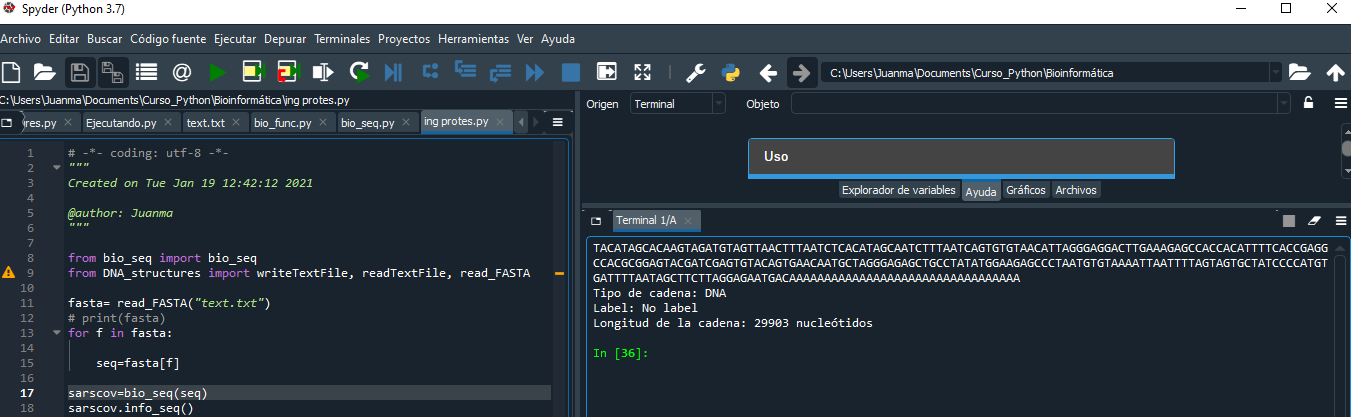
\includegraphics[trim={0 0 0 3cm},clip,scale=0.45]{Screenshot_3}
\end{figure}
Vemos que el genoma del virus cuenta con apenas 30000 nucleótidos. No deja de resultar paradójico cómo una secuencia genética tan ínfima, y que de hecho cabe en apenas un par de páginas de los procesadores de texto, ha dado lugar a tan graves consecuencias.
\newline

Otros datos interesantes son los referidos a la proporción de nucleótidos y al contenido en GC
\newline
\begin{figure}[H]
\centering
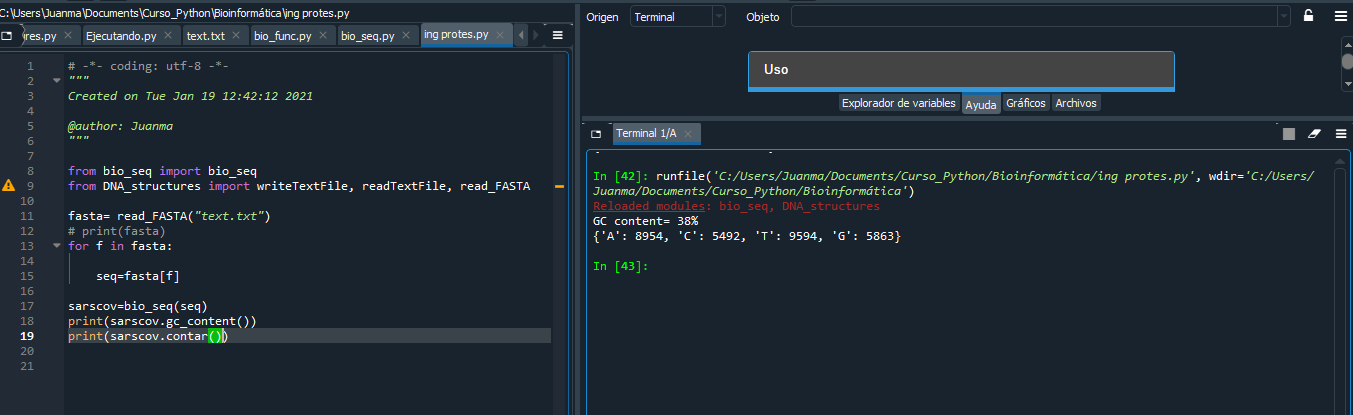
\includegraphics[scale=0.4]{Screenshot_4}
\end{figure}
Es interesante observar que el porcentaje en GC es relativamente bajo. A pesar de que el contenido en GC puede parecer una característica que aporta poca información cada vez son mayores los indicios de que puede tener relación directa con el uso de codones y con la presión selectiva a la que está expuesto el genoma. De hecho, me parece especialmente interesante que este porcentaje se asemeje tanto al que tiene el genoma humano, en torno a un 40 por ciento, lo que me sugiere que determinadas proporciones en GC dan lugar a proporciones y usos de aminoácidos específicos que benefician la replicación del virus, ya que este debe ser procesado por la célula hospedadora. 
\newline

Es más, determinados estudios indican que este porcentaje en GC está claramente optimizado y coincide con los porcentajes observados para los genes que más se expresan en el epitelio pulmonar. De esta forma, el virus habría conseguido potenciar su replicación en las células de este tejido. \cite{Li20201537}.
\newline

No obstante, tal vez lo más interesante pueda ser obtener la secuencia real del virus, que recordemos es ARN. Supongo que el hecho de que aparezca en “tipo ADN” se debe a la forma de obtención de la secuencia, pues por mis conocimientos entiendo que lo que se realiza es una RT-PCR para posteriormente proceder con la correspondiente secuenciación, pues las metodologías de Next Generation Sequencing aún no están lo suficientemente establecidas para llevar a cabo análisis de secuencia directamente del mRNA. 
\newline

\begin{figure}[H]
\centering
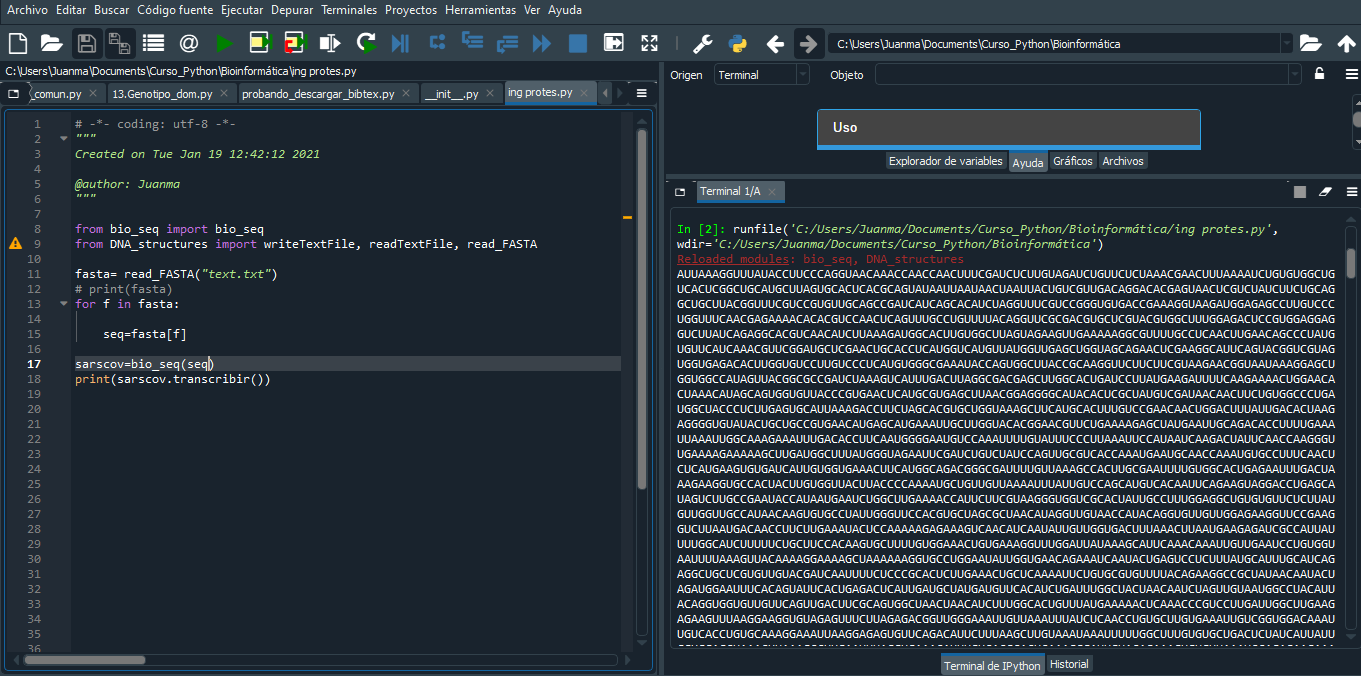
\includegraphics[width=1.2\textwidth]{Screenshot_10}
\end{figure}
Por desgracia, a pesar de ser un virus con un material genético relativamente corto, casi 30000 nucleótidos sigue siendo una cantidad de información enorme, por lo que procederemos a tratar únicamente con la región correspondiente a nuestra proteína de interés, [19621 - 20658]. Ojo, hay que tener cuidado y restar un valor a cada posición, pues Python toma la posición inicial de una cadena como la posición 0.
\newline

\begin{figure}[H]
\centering
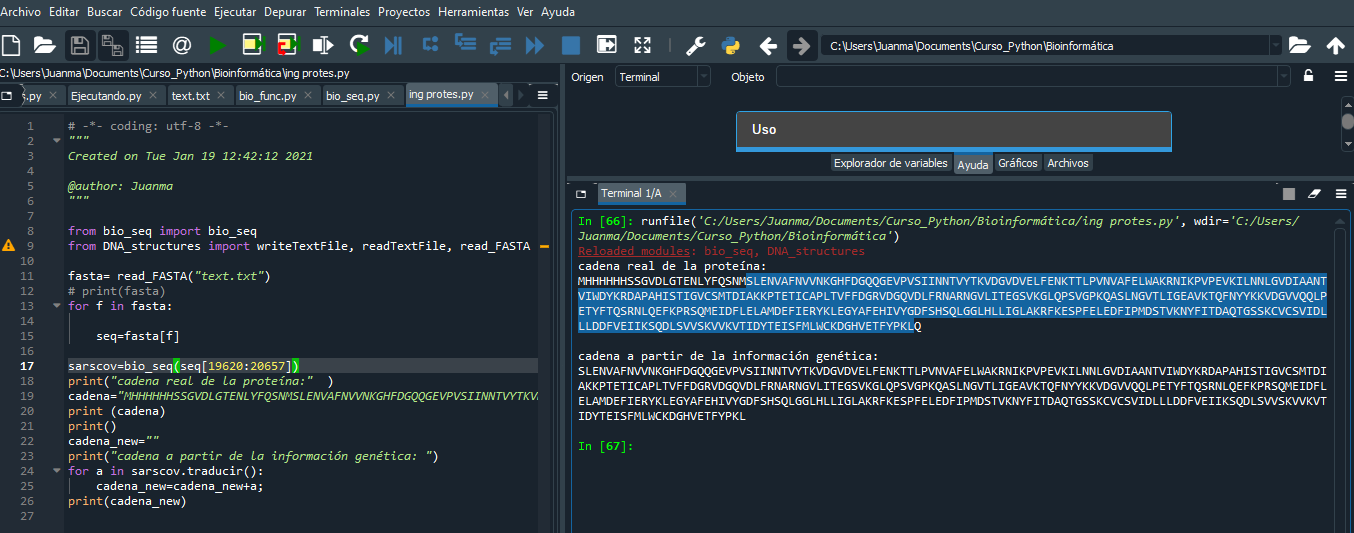
\includegraphics[width=1.2\textwidth]{Screenshot_5}
\end{figure}
Se observa claramente que la proteína sufre ciertos cambios respecto a su secuencia, pero esto no se debe a una modificación o maduración, sino a que en los análisis que se realizan para determinar la estructura de la proteína los datos de los extremos suelen ser de menor calidad y no se tienen en cuenta para la creación del modelo.
\newline

\begin{figure}[H]
\centering
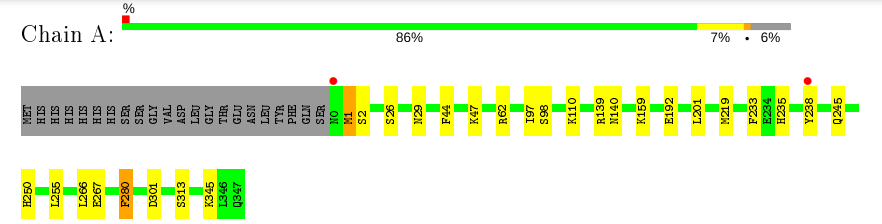
\includegraphics[scale=0.6]{Screenshot_6}
\caption{Imagen obtenida del documento correspondiente a la estructura 6WXC en PDB. Se indican en gris los residuos que no se representan en el modelo.}
\end{figure}


Con este pequeño análisis de la genética del virus hemos demostrado que los datos genéticos y estructurales tienen coherencia, de forma que podemos confiar más si cabe en los datos estructurales de las secuencias de PDB. Por supuesto, no es que yo desconfíe de los datos aportados en PDB, pero considero que una de las cualidades que debe tener todo investigador es la capacidad crítica de análisis de la información, por lo que nunca está de más entender de qué manera se obtienen los datos que se nos presentan para poder darles un uso adecuado. Con este punto de partida, procedemos a analizar los elementos estructurales de la proteína en cuestión.
\newline


Antes de proceder a analizar la estructura y conformación de la proteína cabe destacar que estamos trabajando sobre virus ARN, lo que tiene importantes repercusiones. En virus ARN no se suele hablar de especie, sino de cuasiespecie. Esto se debe a que en su proceso de replicación hay un gran cantidad de errores, lo que determina tasas de mutación mucho mayores a las observadas en seres vivos y virus tipo ADN, hasta cien mil veces mayores. Esto provoca que simultáneamente podamos encontrar diferencias bastantes significativas entre los genomas de una población de virus, y esto es lo que va a ocurrir con el SARS-COV2. La secuencia genética no se corresponde a una variante predominante dentro de la población, sino a la secuencia consenso que se establece a partir de la estimación de todas las cepas y variantes circulantes. 
\newline

Esto habrá que tenerlo en cuenta para los análisis estructurales, donde sí se posee una secuencia aminoacídica ``real'' obtenida de una de las variantes circulantes. La estructura observada será en sentido estricto la que utiliza el virus, es decir, una representación muy fiel, pero que habrá que ir revisando para tener en cuenta todas las modificaciones que se vayan produciendo. Hasta el momento no ha habido un gran número de mutaciones que se hayan expandido para la proteína NSP15, pero si tuviéramos que valorar otras como es el caso de la spike deberíamos valorar que recientemente se ha reportado un claro aumento en el acervo poblacional de determinadas mutaciones muy relevantes para el proceso de infección y replicación del virus.
\newline

\section{Nsp15: Non Structural Protein 15}

El nombre de esta proteína es el acrónimo de “Non Structural Protein 15” del SARS-COV2. Las proteínas no estructurales, como es de esperar, no forman parte de la estructura en sí misma del SARS-COV2 ( estas proteínas serían la spike, la proteína de la membrana, la proteína de la envoltura y la de la nucleocápsida). 
\newline

De las 27 proteínas identificadas, 16 son no estructurales, y han sido identificadas algunas proteínas accesorias que actúan frente al sistema inmune del hospedador. Centrándonos en las no estructurales sus funciones conocidas son varias y en general relacionadas con el procesamiento de las partículas de virus, si bien para algunas de ellas aún no se ha descrito una función aparente.
\newline

Específicamente, la NSP15, nuestra proteína de interés, se trata de una endonucleasa, es decir, su función es la de realizar cortes en el interior de secuencias génicas. No obstante, el conocimiento que poseemos actualmente sobre esta proteína es aún bastante limitado, lo que unido a sus peculiares características la hacen aún más enigmática.
\newline

Se trata de una riboendonucleasa específica de uridilato-RNA  (del tipo NendoU al tratarse de un nidovirus) que posee un dominio C-terminal catalítico típico de la familia EndoU. Este tipo de proteínas EndoU se encuentran en todos los dominios de seres vivos ( y por lo que parece, también en virus) y suelen tener funciones destinadas al procesamiento de distintos tipos de ARN. Además, actúan sobre ARN de cadena tanto simple como doble, y están presentes en diversos grupos de virus que infectan a vertebrados. 
\newline

Más concretamente producen un corte que crea una estructura fosfodiéster 2’-3’ ciclada dejando un 5’ hidroxiterminal, y aunque inicialmente se pensó que actuaban de forma directa en la replicación viral posteriormente se ha podido demostrar que coronavirus deficientes en esta proteína eran capaces de llevar a cabo su ciclo de replicación. Es por ello que se ha propuesto un mecanismo de acción de la proteína frente al sistema inmune, en el que esta proteína destruye el ARN viral sobrante para que no sea detectado por las defensas del organismo infectado. No obstante, esta proteína es esencial para el correcto proceso infectivo, pues le permite al virus llevar a cabo una estrategia de ``evasión'' del sistema inmune \cite{Kim20201596}.
\newline

La entrada del virus en la célula hospedadora se lleva a cabo a través de la liberación de +gRNA (RNA genómico de sentido positivo) en el citoplasma. Desde aquí, este puede sufrir traducción, transcripción del -gRNA complementario, así como replicación y retrotranscripción. En este proceso la Nsp15 parece tener una función clave, pues permitiría una rápida degradación de las moléculas de RNA, con especial afinididad por las colas 3' poliU, que serían fácilmente detectadas por el sistema inmune del hospedador, desencandenando una respuesta inmune contraria al virus. 
\newline

Respecto a la similitud en la secuencia aminoacídica, se ha demostrado que esta es amplia dentro del grupo de coronavirus (tales como el SARS-COV1 y el MERS) mientras que las diferencias aumentan en gran medida cuando tenemos en cuenta otros virus relacionados.
\newline

Para comprobar esta información podemos utilizar la herramienta BLAST, tomando como secuencia de entrada la que hemos tomado anteriormente en formato FASTA.
\newline

\begin{figure}[H]
\centering
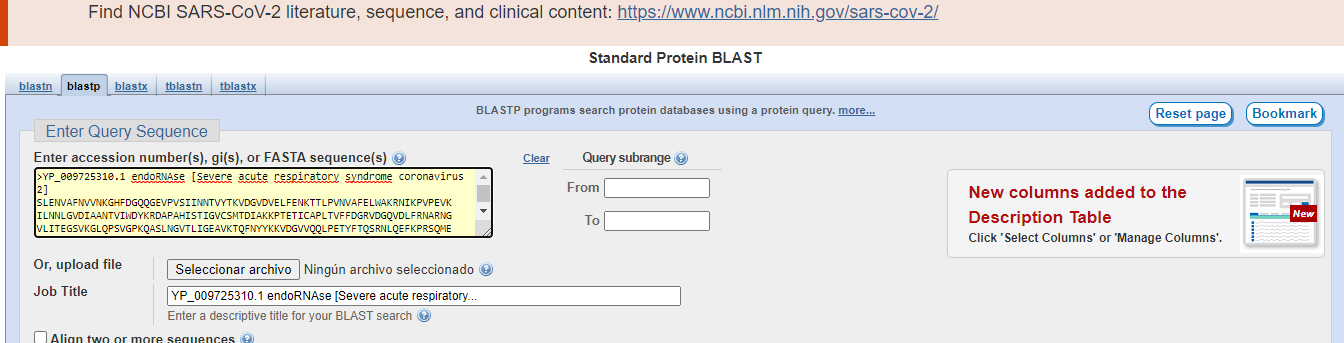
\includegraphics[width=1.2\textwidth]{Screenshot_7}
\end{figure}

Lo primero que nos encontramos al ver las secuencias con mayor porcentaje de similaridad es que hay un gran número de secuencias que corresponden al SARS-COV2. Esto es debido a la inmensa cantidad de análisis que se están realizando sobre este virus, y además nos indica que esta proteína sufre muy pocas modificaciones y que en general, podemos considerar que nuestra secuencia consenso es adecuada.
\newline
\begin{figure}[H]
\centering
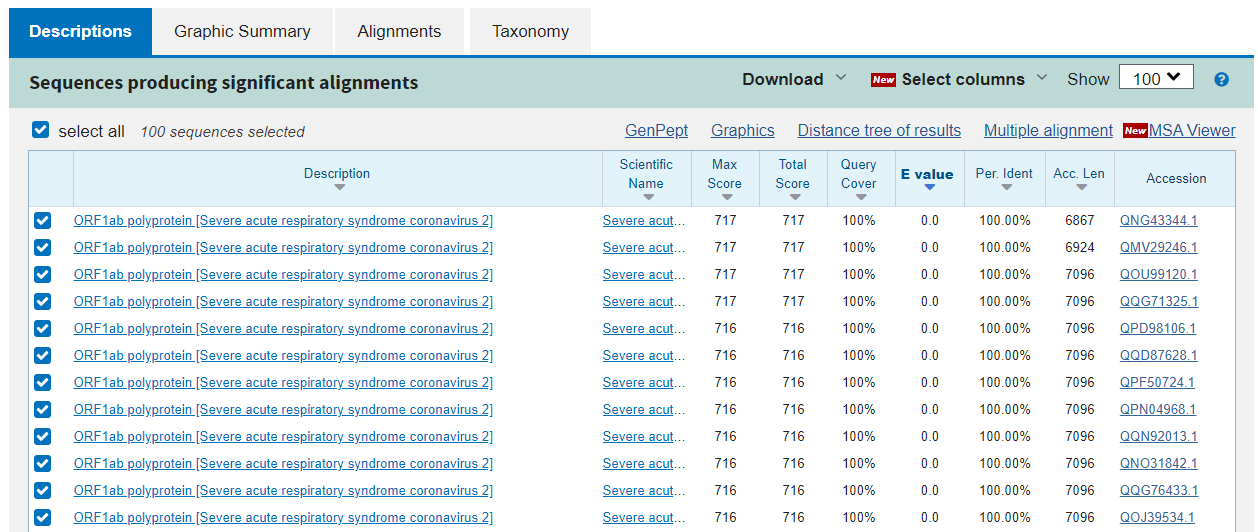
\includegraphics[width=1.2\textwidth]{Screenshot_8}
\end{figure}

Sin embargo, si seleccionamos la opción de que no nos presente las similitudes con otras secuencias de la misma ``especie'', los resultados son aún más interesantes.

\begin{figure}[H]
\centering
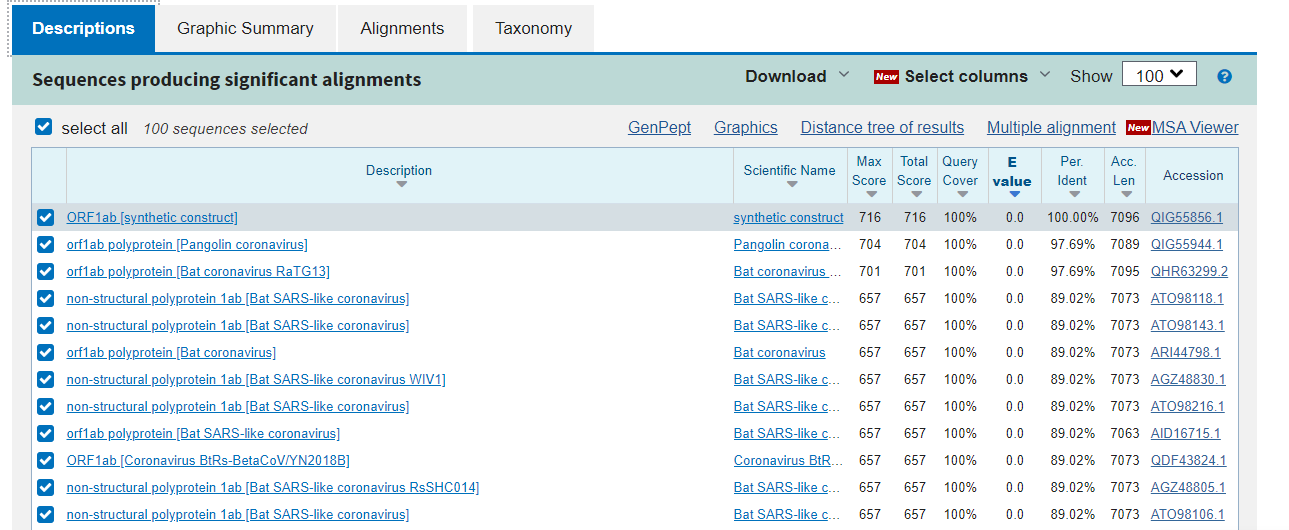
\includegraphics[width=1.2\textwidth]{Screenshot_9}
\end{figure}

Las secuencias más similares y por tanto, más cercanas a nivel filogenético corresponden a coronavirus que infectan a pangolines y murciélagos. Esto es lo que se ha estado defendiendo desde hace meses por la comunidad científica, y con apenas una breve búsqueda hemos podido comprobar en qué se basan para proponer esta hipótesis los expertos que trabajan en este campo de investigación, muy alejados de las teorías conspiranoicas que aseguran sin ninguna base científica que el virus no ha surgido de forma natural. Según los datos recogidos en este somero análisis en BLAST podríamos afirmar que nuestro trabajo tiene cierta coherencia.
\newline

Otro factor interesante a tener en cuenta es que las mayores similitudes no se dan con las secuencias del MERS y SARS-COV1 que crearon ciertos problemas hace unos años, sino con las de coronavirus que infectan a otras especies. Los virus del MERS y SARS-COV1 no consiguieron prosperar como sí lo ha hecho el SARS-COV2, y la clave podría estar en las diferencias genéticas y proteicas que presenta respecto a sus predecesores \cite{Kumar2020}. Por ello, el análisis de la estructura de la proteína lo haremos tomando como punto de referencia las proteínas homólogas de estos virus anteriores, pues a pesar de infectar a humanos no dieron lugar a una emergencia sanitaria como la actual, y podremos inferir los efectos de las mutaciones y diferencias estructurales que podamos observar.
\newline

Más concretamente y centrándonos en nuestra proteína de interés, los cambios no son de una gran envergadura, pero se ha hipotetizado que serían suficientes para contribuir sustancialmente a la virulencia del SARS-COV2.
\begin{figure}[H]
\centering
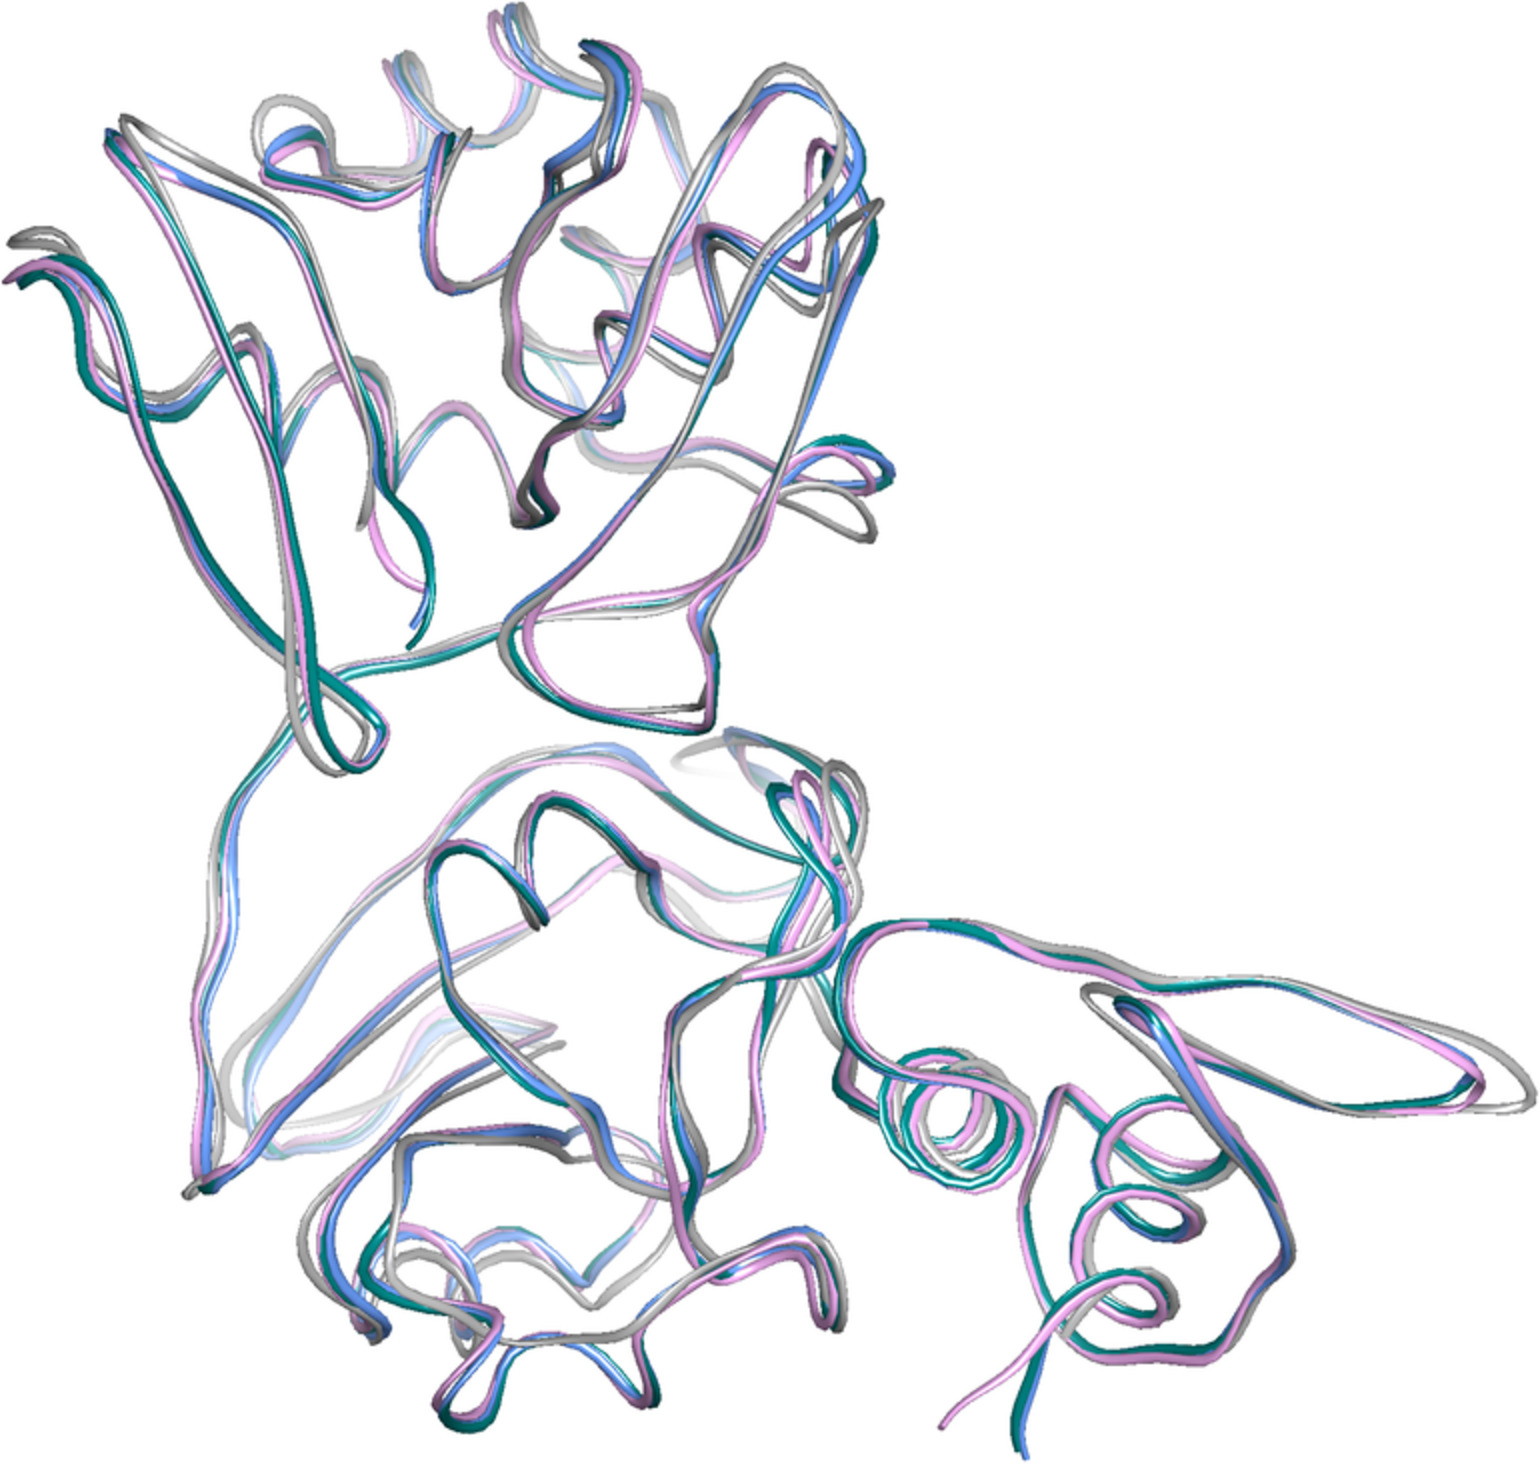
\includegraphics[width=0.8\textwidth, height=12cm]{fig2}
\caption{Superposición de los monómeros de la Nsp15 del SARS-COV2 (en verde azulado), el SARS-COV1 (rosa) y el MERS (gris). Tomada de Kim et at. (2020)  }
\end{figure}

Sin embargo, para poder entender estos cambios primero debemos centrarnos en analizar la estructura de la proteína, entender sus dominios y regiones de interés y posteriormente, inferir la funcionalidad y características de esta secuencia aminoacídica.
\newline

\begin{figure}[H]
\centering
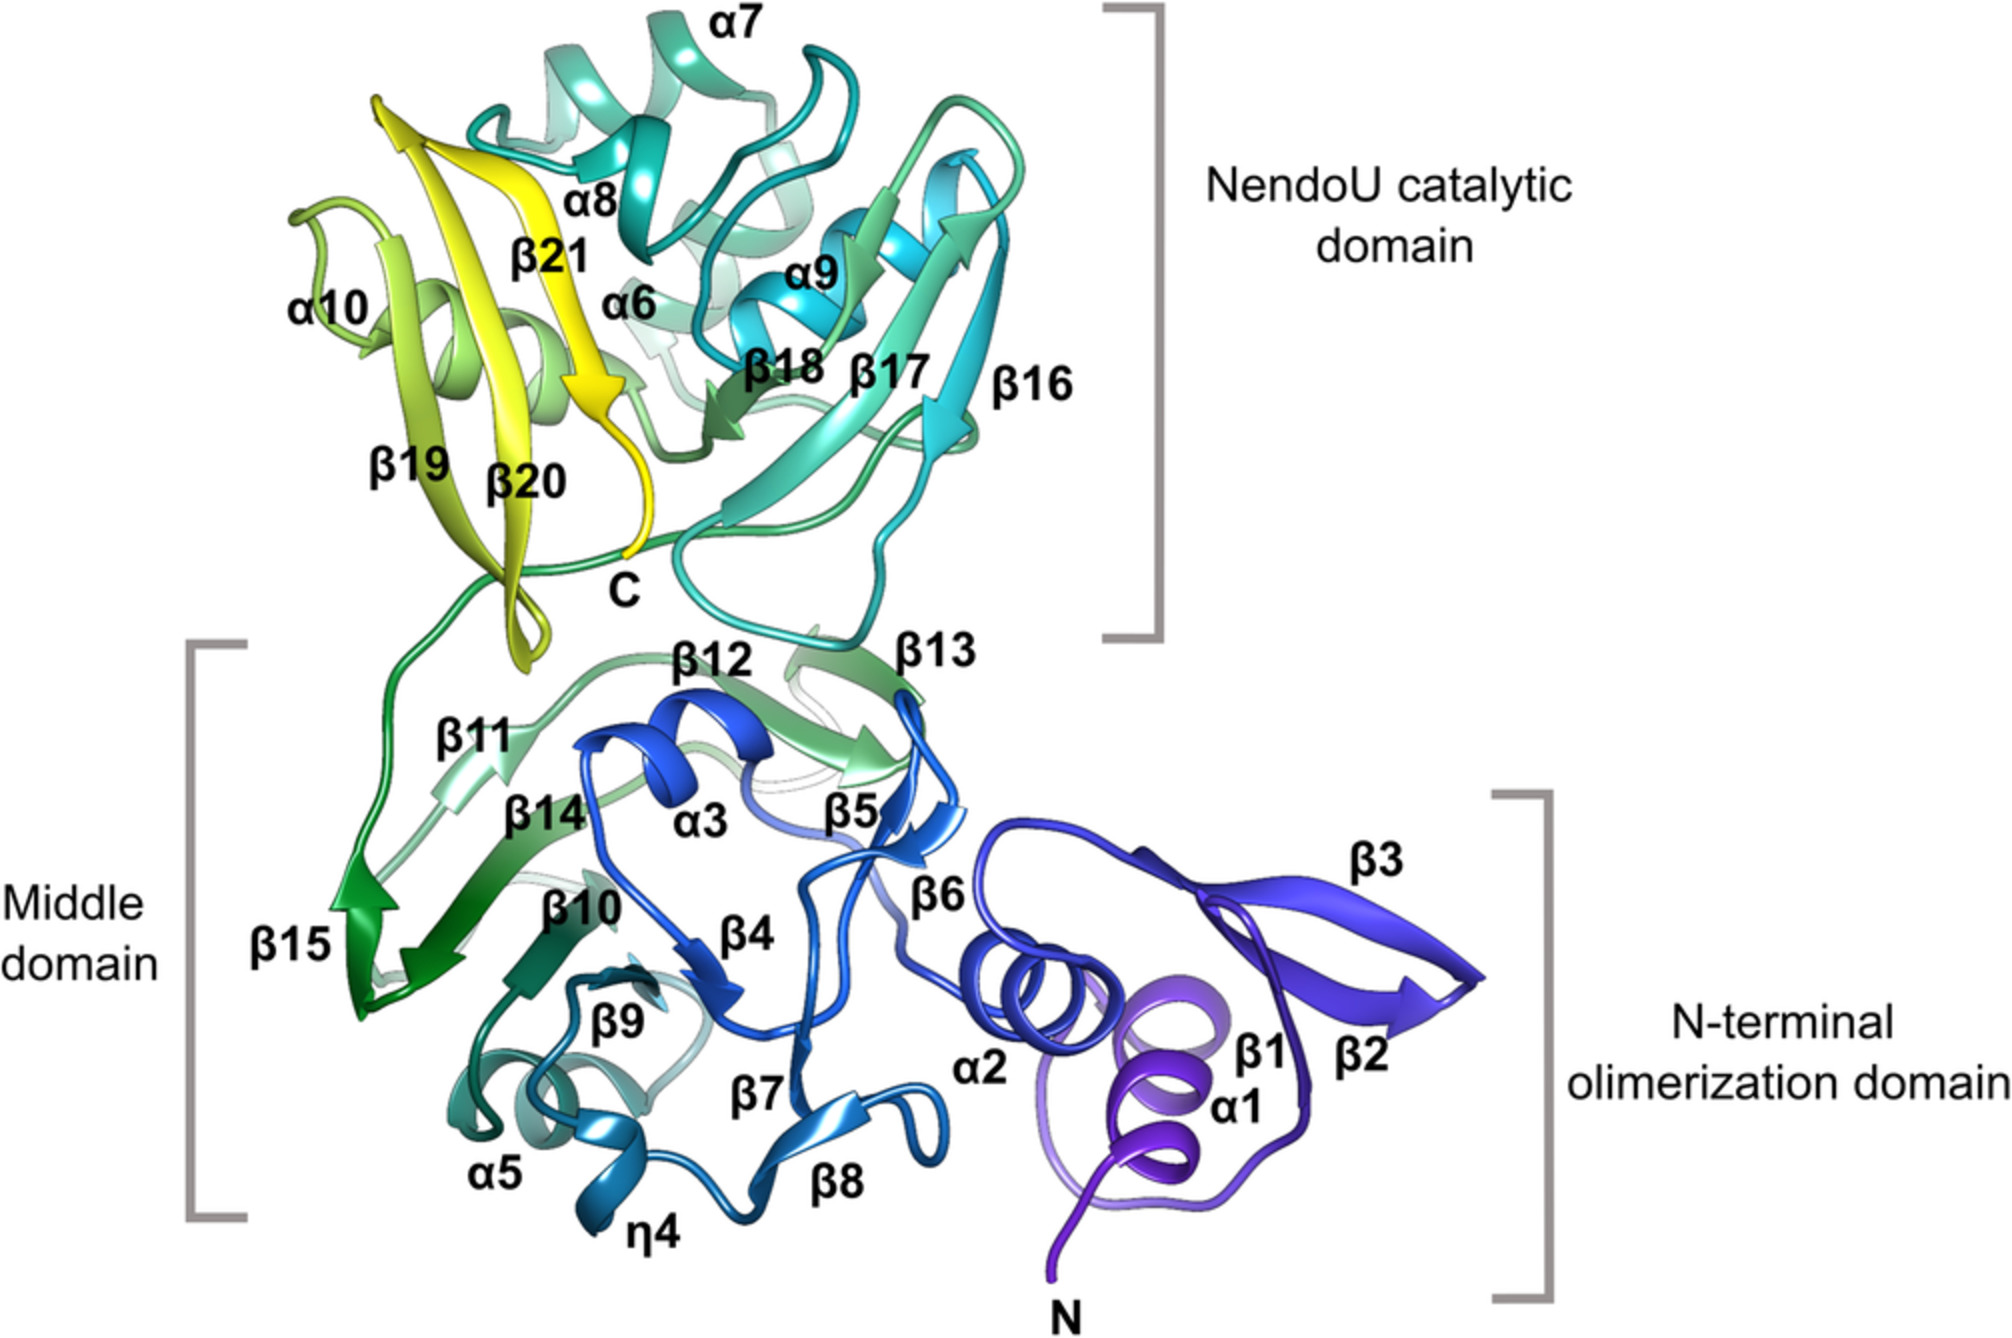
\includegraphics[width=0.8\textwidth]{fig3}
\caption{Estructura del monómero de la proteína Nsp15 con sus principales dominios y regiones estructurales}
\end{figure}
\bibliographystyle{apacite}

Como podemos observar, el monómero presenta 3 dominios principales:
\begin{itemize}
\item 1. Dominio NendoU donde reside la actividad catalítica (C-terminal)
\item 2. Dominio intermedio que une los dominios N y C-terminales.
\item 3. Dominio N-terminal responsable de la formación del hexámero
\end{itemize}

\subsection{Dominio NendoU}
En este dominio es donde reside el centro activo catalítico responsable de la actividad endonucleasa sobre ARN de doble cadena. Más concretamente, en una pequeña hendidura que se encuentra entre las $\beta$ láminas de este dominio, donde destacan 6 residuos (His235, His250, Lys290, Thr341, Tyr343 y Ser294), con una posición y arquitectura conservada entre los 3 coronavirus mencionados a excepción de la Lys290, que varía ligeramente su disposición. \cite{Pillon2021}
\newline

His235, His250 y Lys290 son considerados como la triada catalítica, debido a que sus posiciones concuerdan con la que presenta la ribonucleasa A o pancreática, una ribonucleasa poco específica muy estudiada. Por su parte, la Ser294 y la Tyr343 serían los responsables de controlar la especificidad, pues ocupan la posición de los aminoácidos responsables de esa acción en la ribonucleasa A. De hecho, se ha propuesto que la Ser294 sería la encargada de interactuar con el átomo de $O$ del grupo carbonilo del uracilo a través del $N$ de la cadena principal, mientras que el grupo hidroxilo interaccionaría con el átomo de $N$.

\begin{figure}[H]
\centering
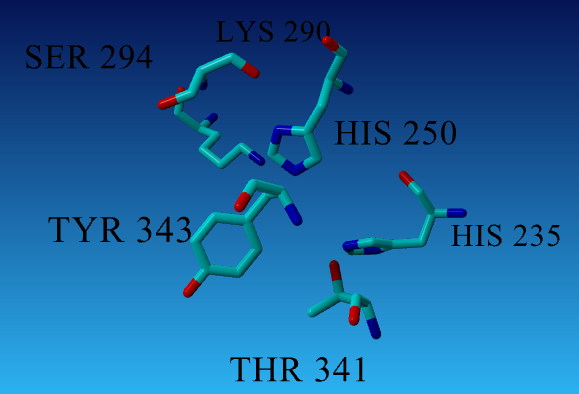
\includegraphics[width=1\textwidth]{Screenshot_12}
\caption{Imagen obtenida del software de visualización YASARA, donde se muestran los principales residuos que forman parte del centro activo con actividad endonucleasa. En la hendidura que se forma se podría introducir el Uracilo con el que se llevaría a cabo la excisión de la cadena ribonucleica.}
\end{figure}

\begin{figure}[H]
\centering
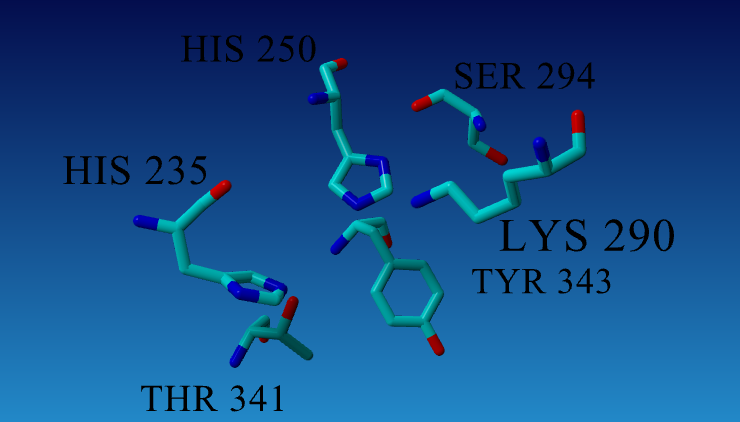
\includegraphics[width=1\textwidth]{Screenshot_13}
\caption{Imagen desde el ángulo opuesto, que nos permite entender la estructura tridimensional del centro activo.}
\end{figure}

\begin{figure}[H]
\centering
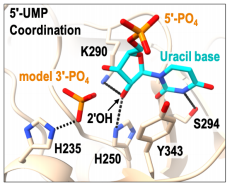
\includegraphics[scale=1.115]{Screenshot_18}
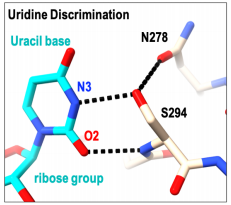
\includegraphics[scale=1]{Screenshot_19}
\caption{Interacción del uracilo con el centro activo de la proteína y su disposición dentro del mismo. Especialmente destacable el papel de la Ser294}
\end{figure}




\subsection{Dominio intermedio}
Se ha hipotetizado sobre la participación de este dominio en la formación del  hexámero (forma activa de la proteína). Al parecer, contribuye a la creación de una estructura cóncava que permitiría la introducción de ARN y proteínas y la interacción de la Nsp15 activa con estos, lo que podría repercutir en una mejora en la actividad catalítica, No obstante, la información es escasa en lo referente a la proteína en su forma hexamérica.
\newline

A pesar de que este pudiera parecer el dominio menos interesante de la Nsp15 es el que presenta un mayor grado de diferencias respecto a sus proteínas homólogas del SARS-COV1 y el MERS. Estos cambios podrían deberse a que no son regiones tan importantes para la función de la proteína y por tanto, no se encuentran tan conservadas. No obstante, ha crecido en importancia la hipótesis de que estas mutaciones podrían tener un papel esencial en el desarrollo de una estructura más eficiente del hexámero. El principal problema para corroborarla, sin embargo, es que no ha sido posible determinar las condiciones necesarias para la hexamerización, si bien existen diversas hipótesis.

\subsection{Dominio de oligomerización}
Debido a las similitudes que presenta la Nsp15 del SARS-COV2 con otras proteínas NendoU se cree que para que se encuentre en forma activa debe formar un oligómero compuesto de 6 subunidades. Para ello, el dominio de oligomerización es esencial, pues a través de este es donde se dan las principales interacciones para tal fin.

\begin{figure}[H]
\centering
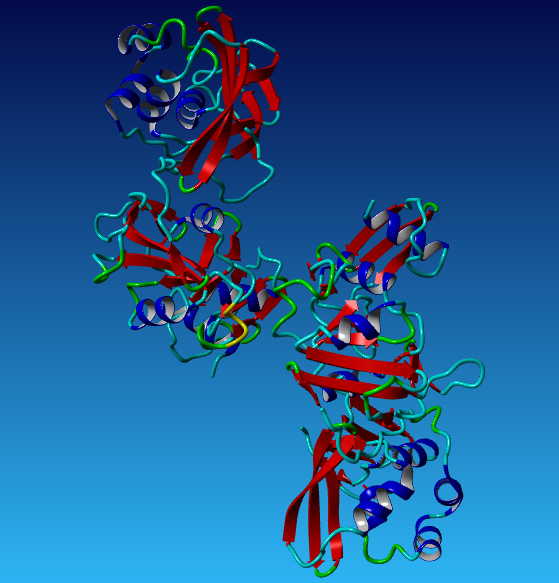
\includegraphics[width=0.9\textwidth, height=12cm]{Screenshot_11}
\caption{Imagen obtenida del software de visualización YASARA, donde se puede observar la interacción entre dos subunidades de la Nsp15 a través del dominio de oligomerización. Las subunidades se disponen en sentido opuesto}
\end{figure}

\begin{figure}[H]
\centering
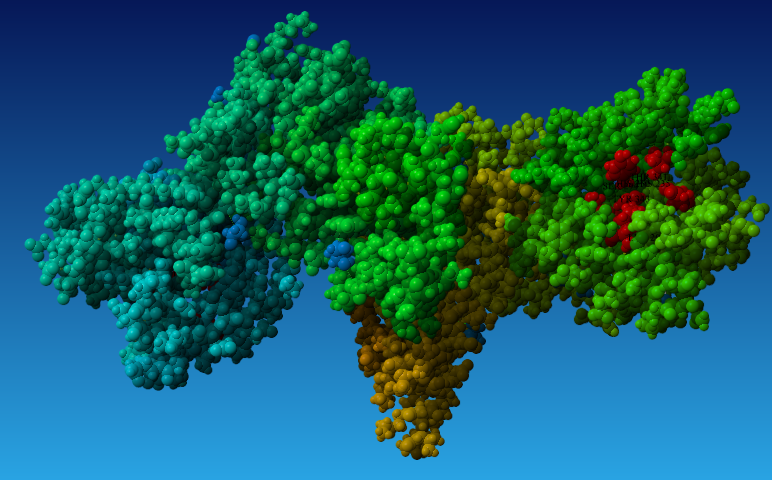
\includegraphics[width=1\textwidth, height=8cm]{Screenshot_15}
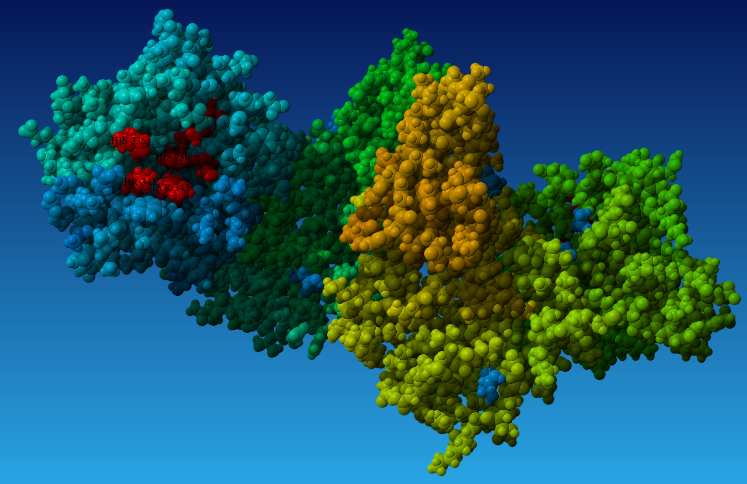
\includegraphics[width=1\textwidth, height=8cm]{Screenshot_16}
\caption{Imagenes obtenidas desde distintos ángulos donde aparecen marcados los residuos del centro activo (rojo), sirviendo de referencia para entender la disposición de los dominios catalíticos de cada subunidad, pudiendo observar la unión por las regiones de oligomerización. Además, se puede observar con gran facilidad la hendidura del centro activo.}
\end{figure}

Por otra parte, las predicciones estructurales parecen indicar que todos los dominios de cada subunidad interaccionan para permitir la formación del dímero de trímeros que constituye la forma activa de la Nsp15. Además, los indicios indican que todas y cada una de las subunidades interaccionan en mayor o menor medida con el resto, lo que crearía una estructura muy compacta.
\newline

Debido a que no se ha encontrado ninguna divergencia importante es las regiones encargadas de la actividad catalítica de la enzima los investigadores piensan que las principales modificaciones en la secuencia y estructura de la proteína han tenido como resultado una mejor disposición de las subunidades dentro del hexámero, lo que repercutiría en una acción más eficiente del complejo en el corte de cadenas ribonucleicas.

\subsection{Hexámero}
La forma hexamérica es la única en la que la Nsp15 presenta actividad. No obstante, y a pesar de que se desconocen las condiciones necesarias para la formación del mismo, se ha propuesto un modelo en el que la activación de la proteína se produce en base a un cambio alostérico en la misma dependiente de la oligomerización. Más específicamente, se ha observado que la oligomerización tendría repercusiones en la disposición del centro activo, restringiendo su movilidad y por tanto, el número de estados posibles. 
\newline

Además, se ha observado que la unión de UMP modifica la arquitectura del centro activo, estableciendo aún más similitudes con la bien estudiada ribonucleasa A, si bien parece ser que daría lugar a una estructura con una capacidad catalítica relativamente lenta.
\newline

Esto tiene vital importancia. El dominio NendoU tiene una alta movilidad, similar a un balanceo. Se cree que esto permitiría una rápida unión a las moléculas de ARN, mientras que la reacción sería lenta. Esto facilitaría una retirada rápida de moléculas que podrían ser reconocidas por el sistema inmune del hospedador. No obstante, también hay indicios de que este balanceo pueda ser clave en la comunicación con el resto de subunidades que forman el hexámero, a través de cambios alostéricos. De hecho, la hipótesis más aceptada actualmente indica que la estructura en hexámero con disposición simétrica en un anillo de dímero de trímeros sería el punto de partida para un mayor número de conformaciones, todas ellas asimétricas, que permitirían la unión a diferentes puntos de un mismo ARN. 
\newline

De esta manera sería posible explicar que la conformación en hexámero sea la única activa para la proteína Nsp15. No obstante, aún quedan muchas cuestiones sin resolver. Entre ellas, destacan algunas referentes a si todos los centros activos realizan cortes o si simplemente pueden servir de anclaje, lo que permitiría un corte más específico en la longitud de las colas poliU, o incluso el ya mencionado problema sobre cómo se forma este hexámero y en qué condiciones lo hace. A pesar de que se han descrito numerosos ligandos y moléculas capaces de unirse a la proteína, su acción sigue sin estar clara, lo que le añade aún más misterio a esta estructura.
\begin{figure}[H]
\centering
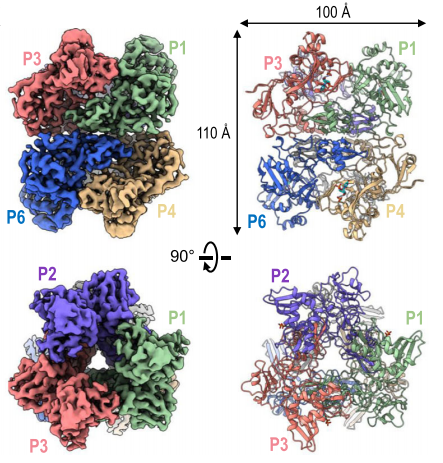
\includegraphics[scale=0.8]{Screenshot_20}
\caption{Estructura en anillo de dímero de trímeros descrita para la Nsp15. Obtenida de Pillon et al. (2021)}
\end{figure}


\section{Opciones terapéuticas}

Debido a la situación de crisis sanitaria, gran parte de la comunidad científica se ha volcado en el desarrollo de medicamentos y vacunas para hacer frente al SARS-COV2. 
\newline

En torno a la casuística de nuestra proteína en estudio, el desarrollo de una vacuna no parece adecuado, pues no se trata de una proteína estructural, por lo que esta opción quedaría descartada. Más aún si comparamos con otras proteínas presentes en el SARS-COV2 como puede ser la spike, protagonista en las diversas vacunas que están superando los ensayos, consiguiendo su aprobación y llegando al mercado.
\newline

Sin embargo, el desarrollo de medicamentos que tengan como target la Nsp15 sí que se ha valorado y existen diversos estudios al respecto. En general, las ribonucleasas son proteínas ampliamente presentes en las células humanas y cumplen diversas funciones, por lo que no será posible la utilización de un inhibidor general de endoribunocleasas. En su lugar, se debe buscar una mayor especificidad, con el objetivo de no alterar el resto de procesos de las células humanas, pues esto podría suponer una fuente de toxicidad e inhabilitaría su utilización terapéutica.
\newline

No obstante, como hemos visto previamente, el centro activo de la enzima se asemeja en gran medida a la ribonucleasa A, que precisamente es una de estas riboendonucleasas de acción general. A pesar de esto he logrado encontrar algún estudio en el que tratan de utilizar inhibidores de ribonucleasa A in vitro para probar su eficacia frente a la Nsp15 del SARS-COV1 y obtienen resultados \cite{Alcantara}. Por desgracia, creo que no se ha tenido en cuenta la posible toxicidad de dichos compuestos y no se han realizado más ensayos al respecto, por lo que dudo de su posible aplicación. Por ello, considero que la especificidad y mejores resultados vendrán dados por la unión que determina la Ser294 que hemos mencionado previamente en este informe. El objetivo será obtener un medicamento que actúe como competidor de las cadenas de RNA con alto contenido en uracilo.
\newline

De esta manera, sería posible en un paciente con la infección activa disminuir la capacidad del virus para ``esconderse'' del sistema inmune, dejando libre gran cantidad de ARN exógeno que se podría reconocer como extraño y desencadenando una respuesta inmunológica adecuada para contenerlo y evitar el desarrollo de síntomatología grave.
\newline

\subsection{Saikosaponinas}
Las saikosaponinas son derivados del oleanano, un triterpenoide natural, que han sido ampliamente utilizadas en la medicina tradicional oriental. Se obtenían principalmente de plantas, siendo ingeridas a través de infusiones y su acción terapéutica frente a virus ha sido constatada en multitud de ocasiones. 
\newline

Para hacer frente a la COVID-19 se han realizado estudios in silico, tratando de determinar si algunas de estas saikosaponinas podrían servir como inhibidoras de determinadas proteínas del SARS-COV2, es especial de nuestra Nsp15. Especialmente destacable es el caso de saikosaponina V, con la cual se observó que podía unirse al centro activo de la Nsp15, bloqueando por consiguiente la unión de cadenas de ARN, y complicando al virus su acción de evasión del sistema inmune. Adicionalmente, cabe destacar que se observó que esta saikosaponina junto con la de tipo U podrían unirse también a la proteína spike e impedir su función \cite{Saurabh}. De ser exitosa esta estrategia su potencial sería enorme. Por una lado inhibiría la entrada del virus a la célula, y por otra permitiría el reconocimiento del ARN viral desencadenando la respuesta inmune pertinente. 
\newline

\begin{figure}[H]
\centering
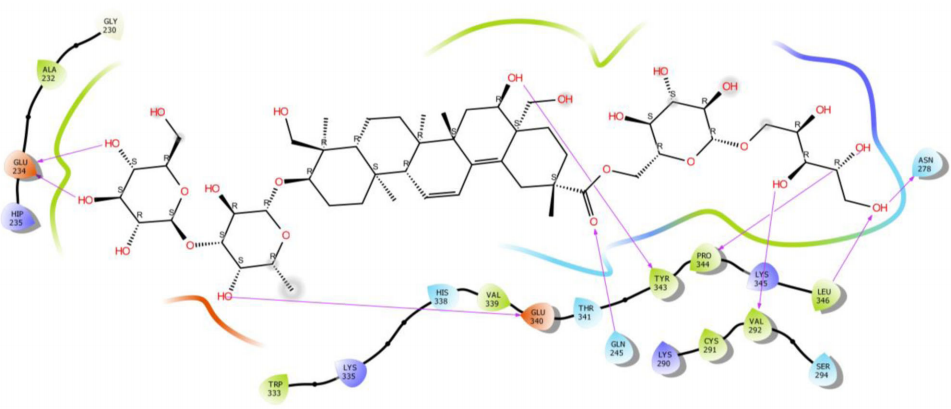
\includegraphics[scale=0.65]{Screenshot_22}
\caption{Representación de las interacciones planteadas entre la saikosaponina V y la Nsp15. Sinha y cols. (2020)}  
\end{figure}


No obstante, cabe destacar que se trata de un estudio in silico y que debería replicarse en condiciones de laboratorio para confirmar su efectividad.
\newline

Siguiendo esta línea de investigación se han propuesto diversos compuestos químicos derivados de plantas para hacer frente al SARS-COV2. De hecho, en este ámbito la bioinformática está desempeñando un papel crucial, pues está permitiendo obtener un gran número de resultados de posibles interacciones entre moléculas a través de software de auto-docking \cite{Savale2021} \cite{Batool2021}, lo que nos permite hacer un screening inicial de posibles candidatos. Gracias a esta estrategia se han propuesto diversos compuestos útiles: demetoxicurcumina, quercetina y miricetina entre muchos otros. \cite{aniket} \cite{KUMAR2020153317} \cite{Umar2021} 
\newline

No obstante, no he encontrado información referente a ensayos clínicos con estos compuestos, por lo que entiendo que se están tomando en cuenta otras vías prioritarias. Aún así, es importante continuar con estas investigaciones, pues estamos observando nuevas mutaciones en el SARS-COV2 que amenazan a la efectividad de las vacunas, y tampoco sabemos cuánto tiempo va a permanecer el virus entre nosotros.

\subsection{Tipiracil}
El tipiracil es un análogo sintético del uracilo, aprobado desde hace ya un tiempo por la FDA para el tratamiento del cáncer colorrectal que presenta una potencial aplicación frente a la Nsp15 \cite{Kim2020.06.26.173872}.
\newline

La estrategia es simple, el tipiracil podría actuar como inhibir competitivo del uracilo y unirse al centro activo de la proteína, lo que impediría el ingreso de las cadenas de RNA y por tanto, dificultaría la evasión del sistema inmune al SARS-COV2. Con técnicas de molecular docking los resultados eran esperanzadores, y se provó su funcionalidad in vitro, obteniendo una ligera disminución en la replicación del virus. Puede no parecer un gran comienzo, pero la realidad es que ahora mismo no existe ningún medicamento con acción terapeútica real contra la COVID-19 cuando esta se encuentra activa en el paciente, por lo que seguir investigando con este compuesto podría llevarnos a, al menos, tener una manera de mitigar la enfermedad en determinados pacientes. 
\newline

\begin{figure}[H]
\centering
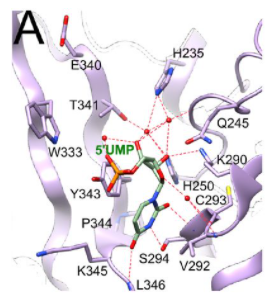
\includegraphics[scale=0.9]{Screenshot_23}
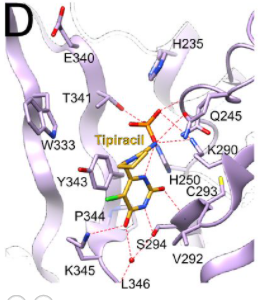
\includegraphics[scale=0.9]{Screenshot_24}
\caption{Comparación de la unión del UMP y el tipiracil}  
\end{figure}

\begin{figure}[H]
\centering
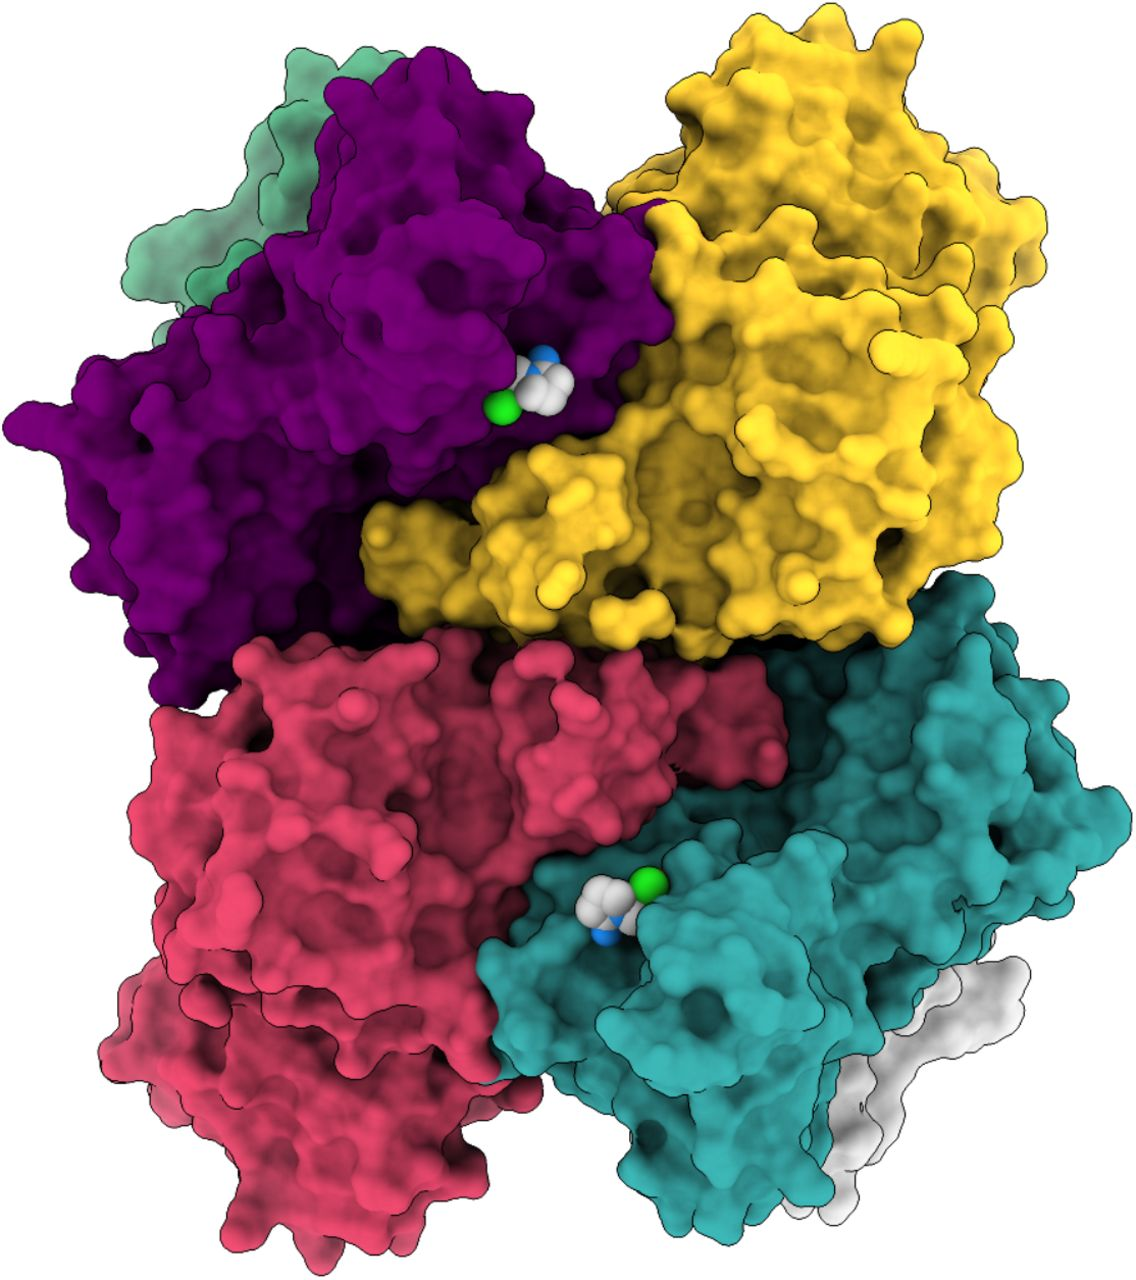
\includegraphics[scale=0.9]{Screenshot_25}
\caption{Unión del tipiracil a los centro activos de la proteína en su forma hexamérica}  
\end{figure}

Al parecer el Tipiracil es capaz de estabilizar los residuos del centro activo, lo que crea una reordenación específica de la proteína. Además, se ha observado una importante acción de la Ser294, tal y como argumentaban otros artículos, en la especificidad de acción de la proteína. Además, parece que la unión a cada centro activo funciona de forma independiente, por lo que sigue sin estar clara la razón por la cuál es necesaria la estructura en hexámero para la funcionalidad de la proteína. En definitiva, el tipiracil puede suponer una importante opción de cara a combatir la infección por el covid.

\subsection{Ciclenosida}
Este compuesto químico es un glucocorticoide inhalado. Este tipo de moléculas se plantearon para hacer frente a la COVID-19 por una doble vía. Por un lado para hacer frente a la replicación del coronavirus, y por otra para disminuir la inflamación del paciente, provocada por la llamada "tormenta de citoquinas". Dentro de los esteroides que se han estudiado, la ciclenosida mostró una baja toxicidad y una capacidad notoria en la disminución de la replicación viral, y además lo hacía de forma específica contra los coronavirus y no contra otros como la gripe, lo que aporta una mayor seguridad sobre su especificidad. \cite{Matsuyama2020.03.11.987016}
\newline

Se observó también que una determinada mutación en la Nsp15 creó resistencia al tratamiento con ciclenosida in vitro, lo que permitió proponer un mecanismo de acción donde la ciclenosida actúa sobre esta proteína, ya sea directa o indirectamente.
\newline

Estudios posteriores in silico han tratado de descifrar la acción de la ciclenosida, observándose una posible unión al sitio catalítico, en contra a otras hipótesis que indicaban una posible acción sobre el dominio de dimerización en la formación del hexámero \cite{pmid32593491}.
\newline

\begin{figure}[H]
\centering
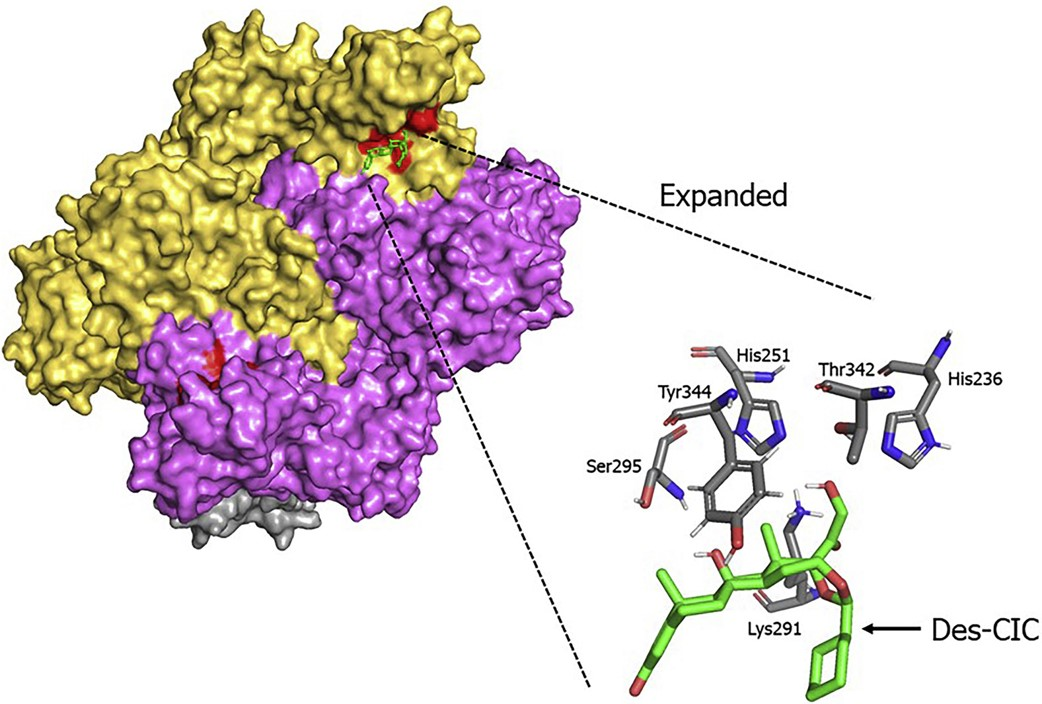
\includegraphics[scale=0.75]{Screenshoot_26}
\caption{Unión de la ciclenosida al centro activo de la Nsp15}
\end{figure}

A pesar de todo, el mecanismo sigue sin estar claro, y el hecho de que se inhiba relativamente la replicación viral sigue sin dejar claro si esto se produce directamente por acción de la ciclenosida, o de forma indirecta por exposición al sistema inmune. No obstante, hay voces que apuntan a que la Nsp15 podría actuar por una doble vía, modificando RNA para mejorar su procesamiento y a la vez destruyendo el exceso para evitar una respuesta inmunológica.


\section{Actividades}

\subsection{Bases de datos secuenciales y estructurales}
\subsubsection{Diagrama de flujo}
El primer ejercicio consiste en la realización de un diagra de flujo que nos permita distinguir entre distintos tipos de archivos, donde destacamos 4 de los más importantes utilizados por la comunidad científica en lo referente a la secuencia y estructura de proteínas: EMBL, Uniprot, GenBank y PDB. Para ello debemos estudiar la estructura y formato que siguen este tipo de archivos. Las diferencias entre ellos serán las que nos permitirán discernir entre cada tipo de archivo, y crear unos comandos lógicos para que nuestra aplicación pueda responder adecuadamente al tipo de archivo que se le indica.
\newline

Si bien podríamos hacer una gran revisión de la estructura de cada uno de estos cuatro tipos de archivos, nos centraremos únicamente en los que nos permiten su identificación y la determinación de la secuencia.
\newline

Respecto a la elección del tipo de archivo, los parámetros a tener en cuenta son los siguientes:
\begin{itemize}
\item PDB. Su primera línea comienza por ``HEADER''
\item GenBank. Su primera línea comienza por``LOCUS''
\item Uniprot. Su primera línea comienza por ``ID'', y la segunda por ``AC''.
\item Emsemble. Su primera línea comienza por ``ID'', y la segunda por ``XX''.
\end{itemize}

Lo que haremos será proceder a crear una estructura lógica de tipo condicional en Pascal, de acuerdo a la siguiente imagen.

\begin{figure}[H]
\centering
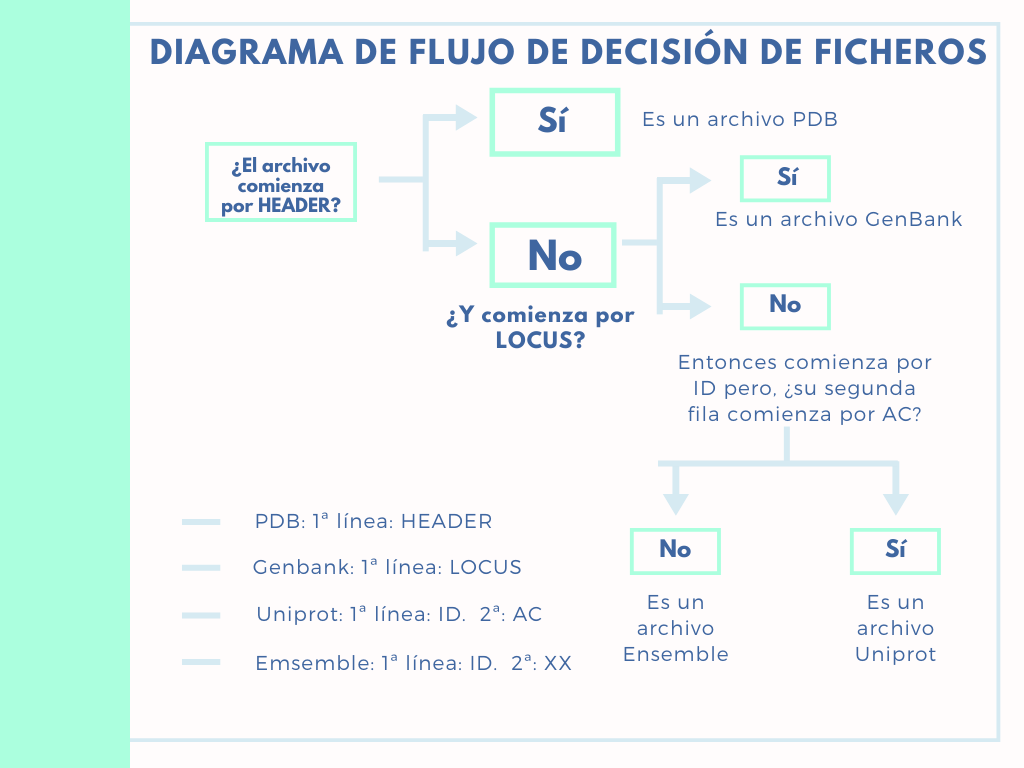
\includegraphics[scale=0.5]{Guía de decisión de ficheros}
\caption{Diagrama de flujo con el que hemos ideado el programa que determina el tipo de fichero}
\end{figure}

Para ello compararemos las líneas del memo que hemos creado con las correspondientes a cada tipo de archivo. Adicionalmente, si no se detecta ninguno de los tipos de archivo el tipo de archivo se queda por defecto como "No detectado", lo que nos permite controlar errores y dirigir al usuario.
\newline

\begin{figure}[H]
\centering
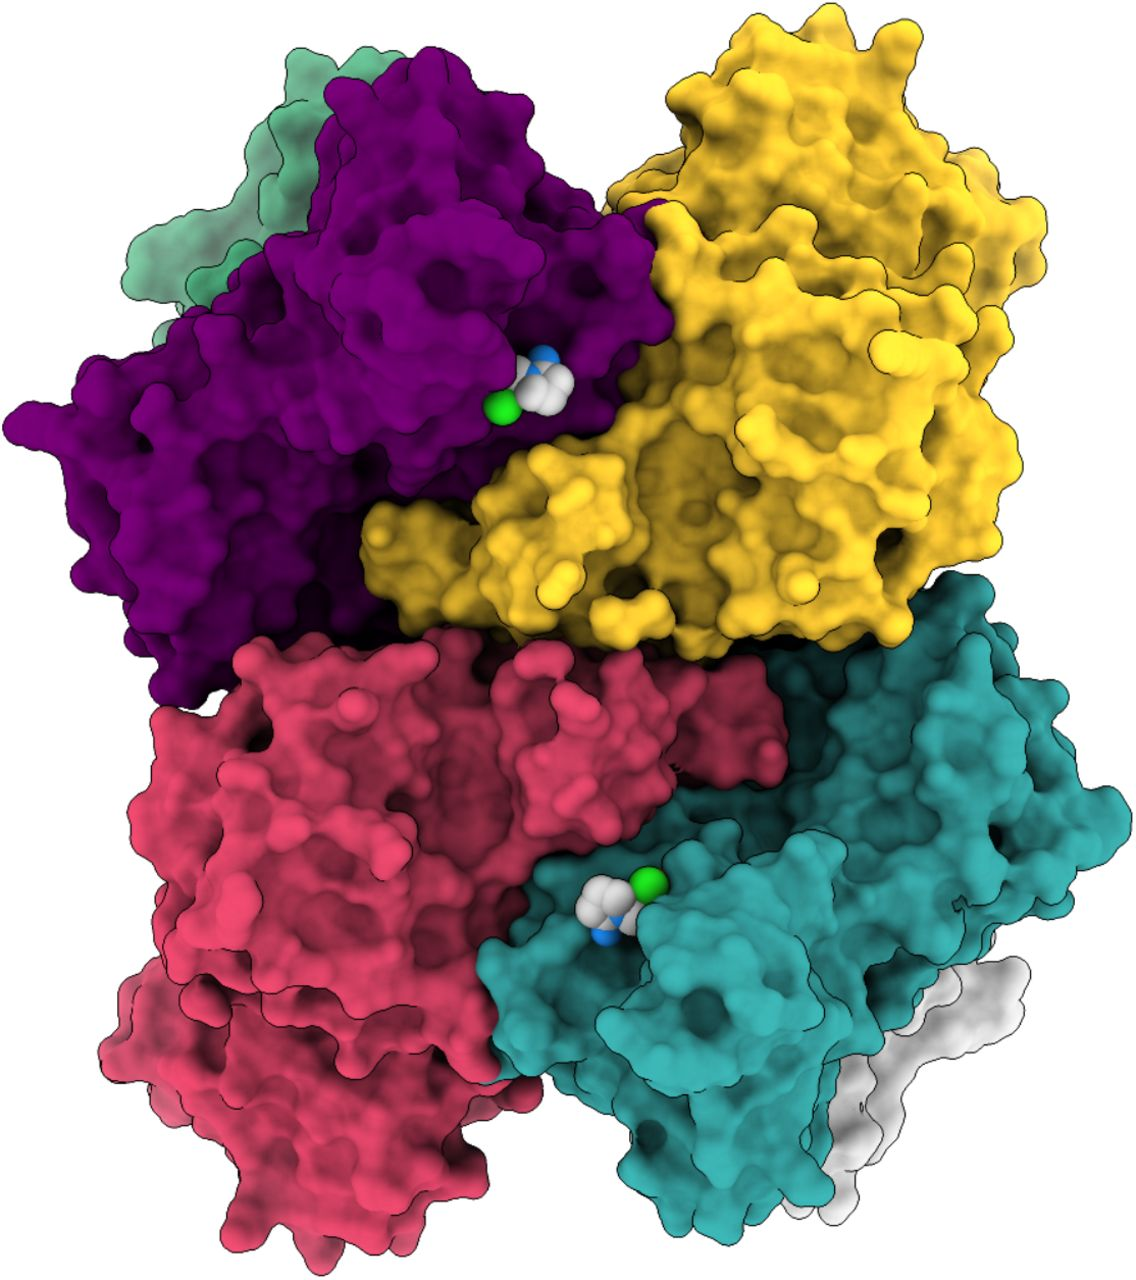
\includegraphics[scale=1]{Screenshot_25}
\caption{Estructura condicional utilizada}
\end{figure}

Paralelamente, se puede obtener la secuencia de la proteína para tres tipos de archivo: PDB, GenBank y Uniprot. Para ello simplemente habrá que utilizar el seleccionador de archivo anterior y delimitar, a partir de la estructura de cada tipo de archivo, obtener la secuencia aminoacídica.
\begin{itemize}
\item PDB. En este caso ya podemos obtener la secuencia gracias a que en Biotools ya habíamos desarrollado esta opción.
\item GenBank. Buscaremos la línea que comienza por ``/translation='', que determina el comienzo de la secuencia, y la línea que comienza por ``ORIGIN''. La secuencia comienza en la prímera línea y termina en la  anterior a la de ``ORIGIN''.
\item Uniprot. En este caso la secuencia está al final del fichero, comenzando en la línea posterior a la que comienza por ``SQ''. Por ello, rastrearemos el memo hasta encontrar esa línea y copiaremos desde la línea siguiente hasta el final del mismo.
\end{itemize}

\subsubsection{Cargar PDB}
Para trabajar adecuadamente con nuestra proteína, necesitaremos leer correctamente su fichero correspondiente. Dentro de los más comunes utilizados en el estudio de proteínas, los archivos de extensión ``PDB'' son probablemente los más utilizados. Estos archivos tienen la características de ser estructurados y contener la información de la posición de cada átomo y la secuencia de la proteína, así como otros datos relacionados con la calidad de la información apartada y cómo se ha obtenido la misma.
\newline

Para aprovechar esta información hemos creado una función denominada ``CargarPDB'', la cual nos creará un objeto de tipo ``TPBD'', que hemos denominado así porque contendrá toda la información relacionada con la estructura y posición de los átomos, los residuos y la subunidad de la proteína.
\newline

Es muy importante conocer la estructura de este objeto, pues va a ser la pieza angular de todas las acciones que realicemos en el resto de aplicaciones y además, será clave para cualquier representación que hagamos ya que alberga toda la información estructural y posicional.
\newline

En líneas generales, está estructurada en tres espacios diferenciados: datos referentes a los átomos, datos referentes a los residuos, y datos referidos a las subunidades, de menor a mayor nivel de complejidad. 
\newline

Para ello, hemos tomado la información de la cadenas que comienzan por ``ATOM'' para la información relativa a los átomos (obteniendo sus coordenadas, código ID, residuo, subunidad, e incluso temperatura). Esto es lo que denominamos TAtomPDB, y que nos permite acceder a las características de cada átomo introducido.
\newline

Tras esto, para los residuos hemos tomado todos los átomos con ID ``N'' cabecera de residuo, es decir, de la cadena principal, los de la cadena lateral tienen otra nomenclatura diferente, obteniendo los ID del residuo de 3 y 1 letra, el nº de residuo y la subunidad a la que pertenece, así como hemos agrupado todos los átomos de ese residuo e incluso sus ángulos $\phi$ y $\psi$ ). Esto es lo que denominados TResiduoPDB
\newline

Por último, hemos creado una estructura que contiene las subunidades a partir de los residuos cabecera de cada subunidad, y que tiene integrada la información necesaria para referenciar a los átomos y residuos de las estructuras anteriores. Esto es lo que denominados TsubunidadPDB.

\begin{figure}[H]
\centering
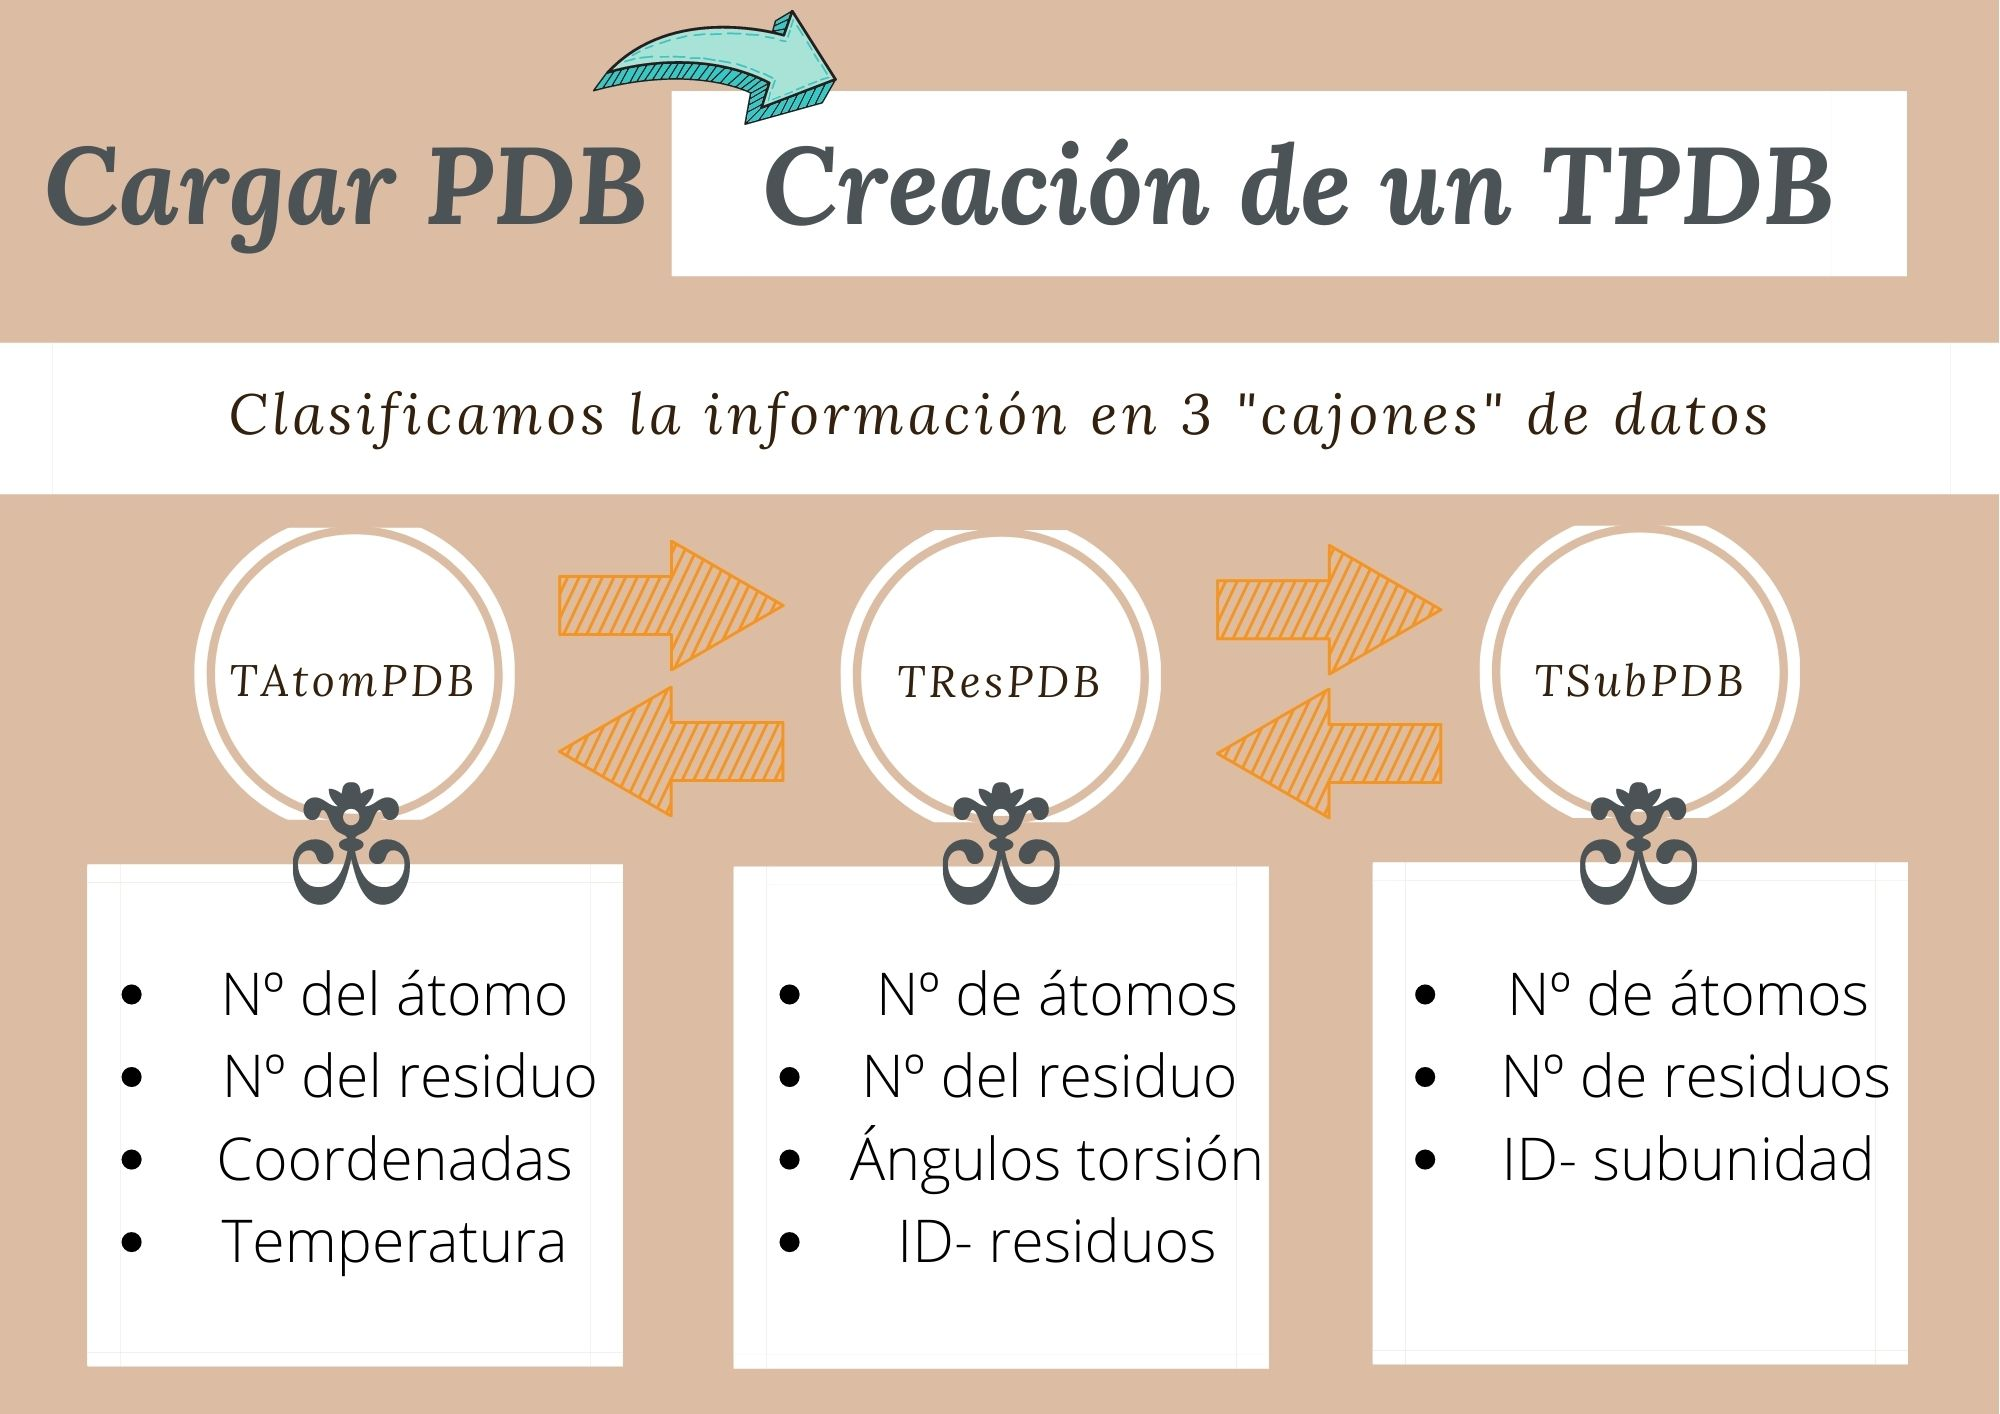
\includegraphics[scale=0.34]{Cargar PDB}
\caption{Utilidad y estructura de la función ``CargarPDB''}
\end{figure}

\subsection{Visualización de proteínas}
\subsubsection{Ficheros de estructuras}
Esta actividad ha sido llevada a cabo de forma paralela a la revisión bibliográfica, utilizando los ficheros ``6VWW'' y ``6WXC'' pues el último archivo ``6X41'' no se encuentra aún disponible en la base de datos del Protein Data Bank. En el apartado Nsp15: Non Structural Protein 15 hemos incluido las imágenes y el análisis de las mismas para complementar la información obtenida en la búsqueda bibliográfica.

\subsubsection{WritePDB}
Lo que trataremos de hacer en esta ocasión, a la inversa que en la función CargarPDB, es tomar los datos de un TPDB, y con ello "recrear" las líneas correspondientes a los átomos, con su misma estructura de forma que puedan ser leídos por un programa de visualización de imágenes. Para ello es clave tener claro cuál es la arquitectura de una línea ATOM de un archivo PDB y así poder respetar los carácteres y espacios de cada parámetro.
\newline

Para ello, de igual manera que hemos trabajado en la actividad para determinar los tipos de archivo, comprobamos la estructura de los ficheros PDB. Además, el ejercicio nos pide exclusivamente seleccionar los C$\alpha$ de la proteína.
\newline

Tras crear la función WritePDB y un par accesorias para crear un encolumnamiento adecuado procedemos a crear una aplicación que nos permite obtener en un memo la secuencia de líneas requerida con los correspondientes C$\alpha$ de la proteína de interés. 

\begin{figure}[H]
\centering
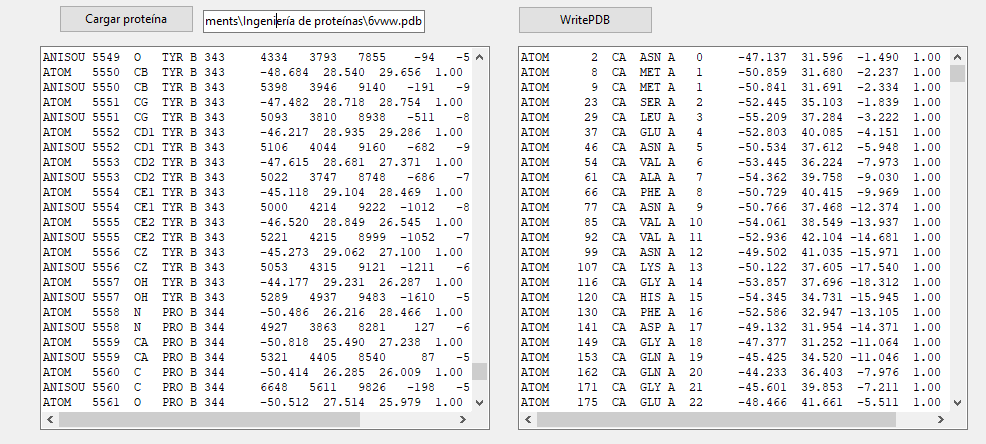
\includegraphics[scale=0.6]{Screenshot_28}
\caption{Aplicación que nos permite obtener las líneas de los C$\alpha$ a partir de la función WritePDB }
\end{figure}

Para certificar que el programa funcionaba correctamente y creaba un archivo válido, utilizamos YASARA y observamos que efectivamente el programa reconoce y representa los átomos que nos interesaban. Para ello es indispensable guardar el archivo con una extensión de tipo ``.pdb'', el archivo en cuestión es ``mod.pdb''.
\begin{figure}[H]
\centering
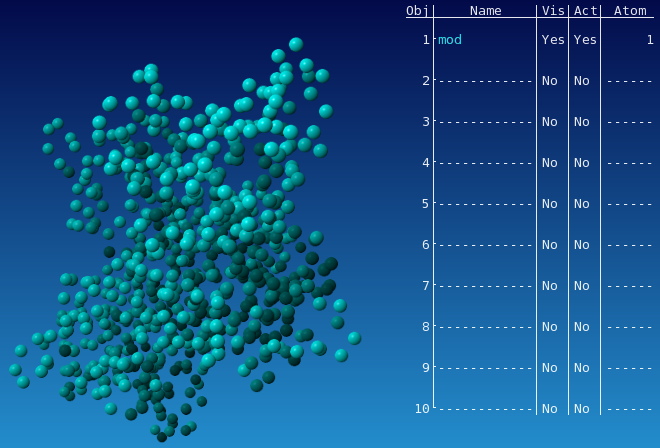
\includegraphics[scale=0.51]{Screenshot_42}
\caption{ Figura obtenida a partir de la representación de los datos obtenidos a partir de WritePDB }
\end{figure}


\subsection{Predicción estructural de proteínas}
\subsubsection{Ramachandran}
Para hacer un diagrama de Ramachandran lo primero que debemos entender es qué son los ángulos de torsión de la proteína.
\newline

Los ángulos de torsión de la proteína son los ángulos llamados $\phi$ (de N a C$\alpha$)  y $\psi$ (de C$\alpha$ a C), que oscilan entre 180 y -180 grados. Estos ángulos de la cadena principal (las laterales en este caso no tiene relevancia) son los que van a determinar la geometría y las propiedades físicoquímicas de la proteína. Adicionalmente, existe otro ángulo de torsión, denominado $\omega$, pero este suele presentar valores establecidos por lo que podremos obviarlo para nuestros cálculos.
\newline

\begin{figure}[H]
\centering
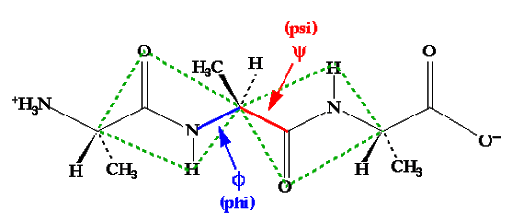
\includegraphics[scale=0.6]{unnamed}
\caption{Representación de los ángulos de torsión}
\end{figure}


Los diagramas de Ramachandran son representaciones de los valores de los ángulos de torsión $\phi$ y $\psi$ de los residuos de una proteína (a excepción del primero y el último, que no poseen ángulos $\phi$ y $\psi$, respectivamente). Estos diagramas tienen una gran importancia a la hora de determinar qué tipo de estructura secundaria es la dominante en la proteína, pues ya se conocen cuáles son las combinaciones de ángulos $\phi$ y $\psi$ que dan lugar a hélices $\alpha$, láminas $\beta$, giros y demás tipos de estructuras. Nuestra tarea consiste en crear un diagrama de Ramachandran de nuestra proteína de interés.
\newline

\begin{figure}[H]
\centering
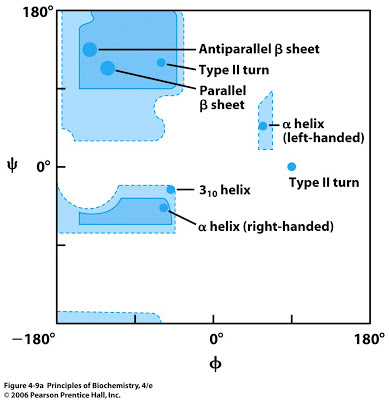
\includegraphics[trim={0 1cm 0 0},clip,scale=0.6]{figurenew}
\end{figure}

Para ello, crearemos los parámetros ``phi'' y ``psi'' en nuestra matriz de datos TResiduosPDB. El valor de estos ángulos será calculado a partir de los átomos de la cadena principal de ese residuo y del anterior o posterior, según trabajemos con $\phi$ o $\psi$.
\newline

Cabe destacar que por convenio se considera al ángulo de torsión como el que forman 4 átomos cuando los dos átomos centrales se encuentran en la intersección de los dos planos que contienen los 4 átomos, formando un diedro. Si observamos la estructura de forma que se superpongan los dos átomos centrales podremos ver el giro existente entre el primer átomo y el último, pudiendo encontrarse superpuestos (cis), en sentido opuesto (trans) y en todas las posiciones intermedias.

\begin{figure}[H]
\centering
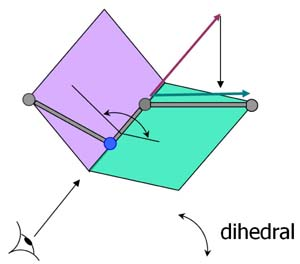
\includegraphics[scale=3]{diedro}
\caption{Perspectiva utilizada para entender los ángulos de torsión.}
\end{figure}

Para calcular los ángulos $\phi$ y $\psi$, necesitábamos las distancias entre los átomos que forman parte del ángulo diedro, para ello utilizamos el vector diferencia $\overrightarrow{v}= \overrightarrow{A}- \overrightarrow{B}$. Asimismo, para calcular el ángulo correspondiente nos valemos de la ecuación del cálculo del producto escalar entre dos vectores. Despejando obtenemos el ángulo de interés

\begin{equation}
\alpha=\arccos\frac{\overrightarrow{v1}\overrightarrow{v2}}{\left\| v1 \right\| \left\| v2 \right\|} 
\end{equation}

De esta manera, aplicada a nuestro caso particular:

\begin{equation}
\alpha=\arccos\frac{(\overrightarrow{A}-\overrightarrow{B})  (\overrightarrow{B}-\overrightarrow{C})}{\left\| \overrightarrow{A}-\overrightarrow{B} \right\| \left\|  \overrightarrow{B} - \overrightarrow{C} \right\|}  
\end{equation}

Observamos que nuestra aplicación Ramachandran funciona correctamente con la proteína que hemos utilizado de prueba durante toda la asignatura ``1AHI'', no obstante, con nuestra proteína asignada nos surgen errores, lo que podría deberse a que el archivo tipo pdb de la misma tiene diferencias respecto a los demás que hemos visto, en especial porque incluye un factor anisotrópico de temperatura y no representa todas las subunidades mencionadas.

\begin{figure}[H]
\centering
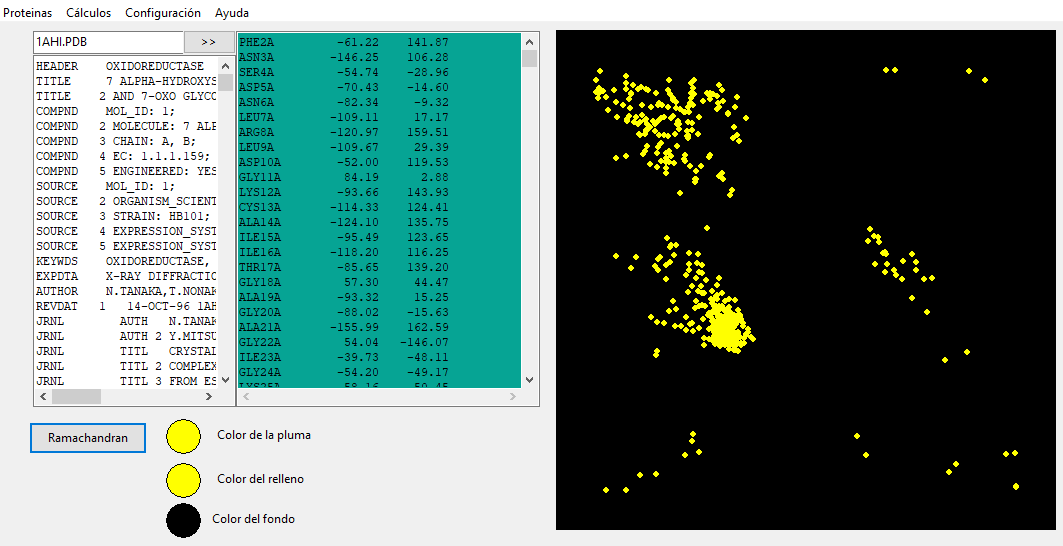
\includegraphics[scale=0.5]{Screenshot_47}
\caption{Perspectiva utilizada para entender los ángulos de torsión.}
\end{figure}

Para poder obtener los valores de los ángulos phi y psi recurrimos a una de las aplicaciones de ``MolProbity'', desarrollada por el departamento de Bioquímica de la Universidad de Duke.
\newline

\begin{center}
\begin{tabular}{| c | c | c |}
\hline
Residuo & $\phi$ & $\psi$ \\ \hline
1 &   -72.92  &  136.32  \\
2 &  -165.55  &  153.42  \\
3 &   -64.36  &  -44.72  \\
4 &   -66.80  &  -29.83  \\
5 &   -72.99  &  -37.85  \\
6 &   -61.97  &  -42.60  \\
7 &   -67.09  &  -32.87  \\
8 &   -59.94  &  -45.86  \\
9 &   -64.99  &  -37.12  \\
10 &  -66.35  &  -43.77  \\ \hline
\end{tabular}
\end{center}

\subsubsection{Coordenadas transformadas}
Durante el progreso de la asignatura hemos creado diversas funciones que nos permiten realizar transformaciones en las coordenadas de los átomos de nuestros TPuntos. Entre estas funciones se encuentran giros sobre los ejes X,Y,Z y translaciones. 
\newline

En conjunto, entre ellas nos permiten realizar modificaciones en la perspectiva con la que vemos la proteína, y como ejemplo visualizaremos la proteína con un giro de 5 grados, lo que nos aporta una pequeña idea de cómo sería la imagen tridimensional de la proteína (considerando como 5 grados el ángulo entre los ojos del observador). En este caso, nos centraremos en la primera fenilalanina y los dos residuos siguientes, representando todos sus átomos correspondientes.
\newline

En otros programas ya hemos realizado representaciones y transformaciones, pero en este caso debemos adaptarlos al residuo requerido, tomando su átomo inicial y el átomo final del residuo n+2 en la cadena. Tomaremos sus coordenadas y crearemos una TTablaDatos para la representación.
\newline

El esquema lógico seguido es el siguiente: se carga un archivo y crea un TPDB, se seleccionan los datos del mismo y se representan los datos con y sin la modificación modificando TTablaDatos. Cabe mencionar que el valor seleccionado para el giro es de ``0.087'' pues es el valor correspondiente a 5 grados en radianes.
\newline

\begin{figure}[H]
\centering
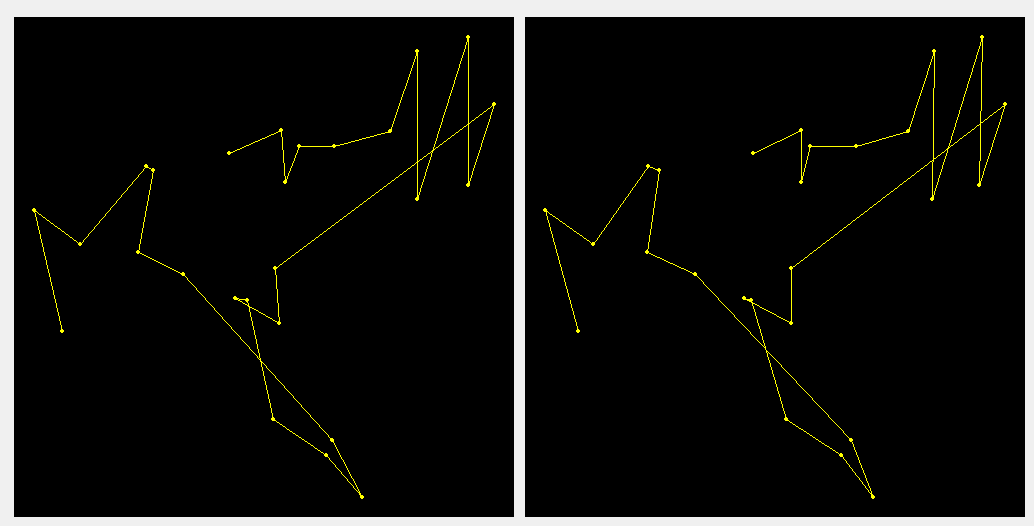
\includegraphics[scale=0.45]{Screenshot_48}
\caption{Imagen obtenida a partir del programa ``Estereodiagrama'' de nuestra proteína de interés. Las diferencias son ligeras debido a que el ángulo de giro es bastante reducido. Imagen modificada a la derecha}
\end{figure}

A pesar de ser un leve giro, se observa la profundidad de la posición de los átomos claramente en algunos átomos. Para asegurarnos de que habíamos realizado bien la aplicación y que el resultado sea correcto comparamos con imágenes obtenidas del software de visualización YASARA.

\begin{figure}[H]
\centering
\begin{subfigure}[b]{0.49\textwidth}
\raggedright
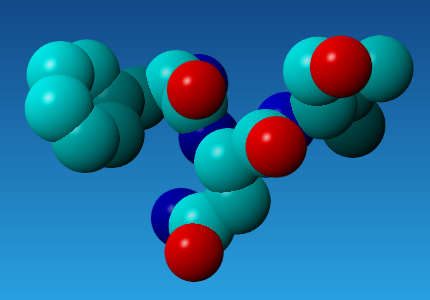
\includegraphics[scale=0.6]{Screenshot_49}
\end{subfigure}
\begin{subfigure}[b]{0.49\textwidth}
\raggedleft
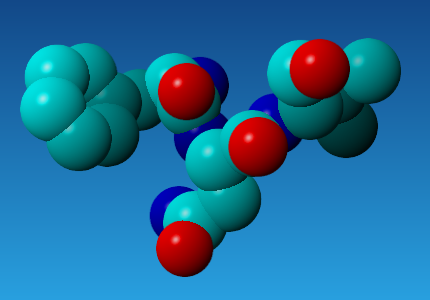
\includegraphics[scale=0.6]{Screenshot_50}
\end{subfigure}
\caption{YASARA, imagen modificada a la derecha. El giro es más leve de ver si cabe debido al tamaño de las esferas correspondientes a cada átomo}
\end{figure}

\subsubsection{Alinear Z}
En esta tarea debemos rotar la proteína para visualizar desde el eje Z. No obstante, para ello hay que colocarla sobre ese eje y de nuevo, deshacer los cambios para obtener las coordenadas adecuadas.
\newline

Para ello lo primero que tenemos que hacer es crear una estructura que nos permite guardar la información relativa a las coordenadas de los átomos de una proteína, esta será llamada TPunto. Con ella, crearemos un array de puntos que denominaremos TPuntos. Ahora ya tendremos toda la información relativa a los átomos de la proteína,y podremos empezar a realizar los cálculos necesarios. En este caso tal y como nos pide el ejercicio solo tendremos en cuenta los C$\alpha$.
\newline

A nivel de cálculos, deberemos realizar las siguientes transformaciones:

\begin{enumerate}
\item Translación de P1 al (0,0,0). Se traslada todo el objeto, incluido el P2. Recordemos que tenemos un eje que une ambos puntos.
\item Giro sobre OX hasta que P2 se encuentre en el plano XZ.
\item Giro sobre OY hasta que P2 esté en el eje Z
\item Giro del número de grados necesario sobre el eje OZ.
\item Inversa del paso 3
\item Inversa del paso 2
\item Inversa del paso 1
\end{enumerate}

Es importante resaltar que en este tipo de transformaciones encadenadas de los giros el orden sí que es importante y es clave mantener una secuencia racional de cambios en las coordenadas de la proteína.
\newline

Para ello tenemos una función ``alinearZ'' que toma un TPuntos y lo devuelve modificado, a través de las siguientes transformaciones:
\newline

En primer lugar realizamos la translación mencionada.
\newline

Posteriormente, realizamos los cambios necesarios al P2 con las siguientes ecuaciones:

\begin{equation}
d1=\sqrt{b^2+c^2}
\end{equation}
\begin{equation}
d2=\sqrt{a^2+b^2+c^2}
\end{equation}

\begin{equation}
sin(\phi)= \frac{cateto opuesto}{d1}
\end{equation}
\begin{equation}
sin(\alpha)= \frac{cateto contiguo}{d2}
\end{equation}

\begin{equation}
\phi=\arcsin(\sin(\phi))
\end{equation}

\begin{equation}
\alpha=\arcsin(\sin(\alpha))
\end{equation}

Finalmente, realizamos los giros correspondientes a los pasos 2 y 3 con los ángulos $\phi$ y $\alpha$ respectivamente. El resto de pasos se omiten para la problemática que se nos presenta. Es decir, obtenemos la representación desde la vista del eje OZ pero sin aplicar los pasos inversos que hemos mencionado anteriormente.
\newline

Respecto a nuestra proteína de interés, la Nsp15, los resultados de los 10 primeros C$\alpha$ fueron los que se muestran en la siguiente imagen:

\begin{figure}[H]
\centering
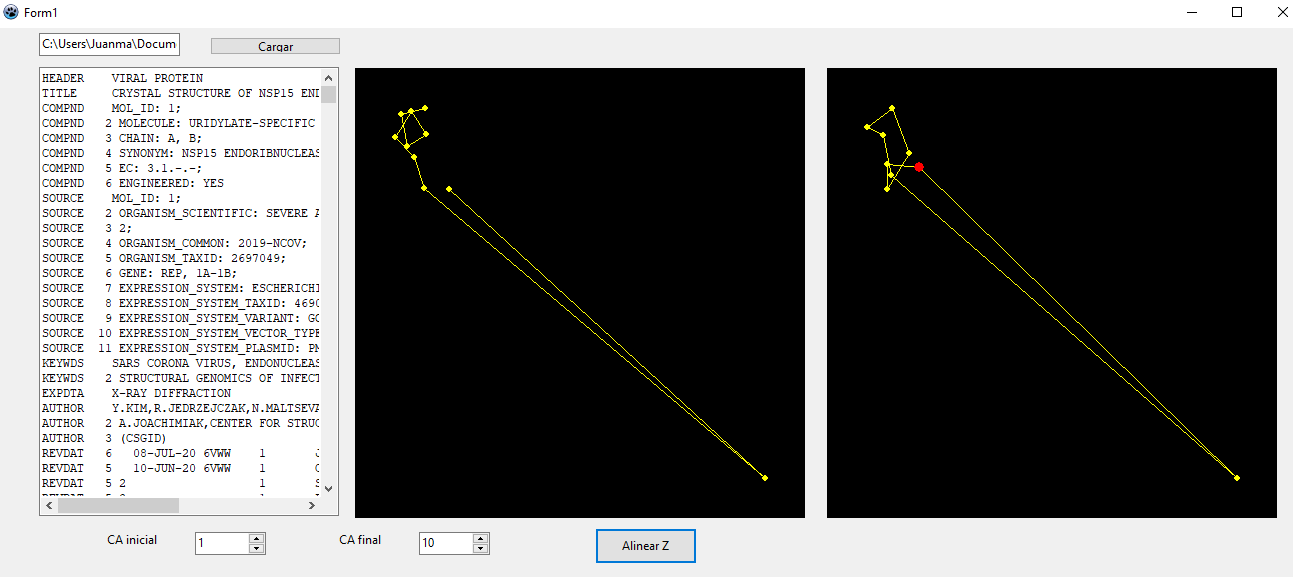
\includegraphics[scale=0.5]{Screenshot_36}
\caption{Imagen obtenida a partir del programa ``alinearZ'' de nuestra proteína de interés. Los átomos superpuestos se muestran en color rojo}
\end{figure}

Simplemente para comprobar que el programa seleccione correctamente los átomos, visualizamos con YASARA los primeros diez C$\alpha$, comprobando que la disposición es similar. Las diferencias se deben a que la vista no es exactamente la misma.

\begin{figure}[H]
\centering
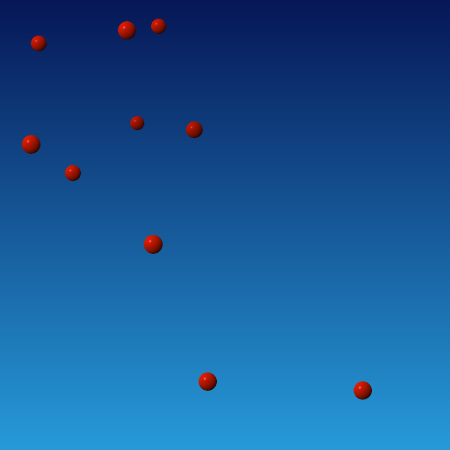
\includegraphics[scale=0.5]{Screenshot_37}
\caption{Imagen obtenida de YASARA}
\end{figure}


\subsubsection{RMSD}

En este ejercicio teníamos que estudiar la diferencia en distancia entre los átomos de las 3 primeras cisteínas de la proteína. Para ello, hemos seleccionado las 3 cisteínas con un bucle que buscaba el código de 3 letras ``CYS'' que presentan estos residuos.
\newline

Tras esto, hemos ido guardando los datos de las distancias entre los átomos en una matriz dinámica, donde los valores de la diagonal deben ser 0 pues un átomo consigo mismo no puede tener un valor diferente para este parámetro.
\newline

Tras esto, hemos calculado los ``dij'' como la suma de las distancias entre los átomos de cada cisteína (átomos obtenidos a partir de los TResiduoPDB), y por último hemos calculado las diferencias entre cada una de las cisteínas, es decir, nuestro RMSD.
\newline

\begin{figure}[H]
\centering
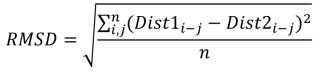
\includegraphics[scale=0.8]{formula1}
\caption{Fórmula utilizada para el cálculo de los valores del RMSD de las cisteínas. Donde n=6 y las distancia son las obtenidas a partir del programa ``RMSD''}
\end{figure}

Por ejemplo, obtenemos los valores correspondientes al RMSD de la siguiente proteína:

\begin{figure}[H]
\centering
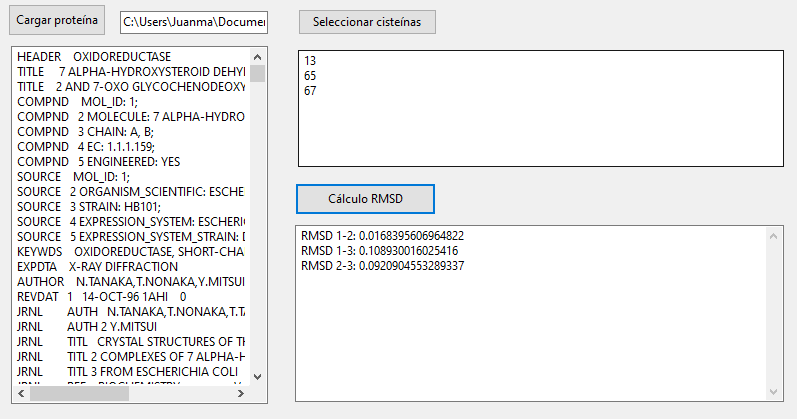
\includegraphics[scale=0.8]{Screenshot_43}
\caption{Fórmula utilizada para el cálculo de los valores del RMSD de las cisteínas. Donde n=6 y las distancia son las obtenidas a partir del programa ``RMSD''}
\end{figure}

\subsubsection{Mutación}

En esta actividad se nos plantea la siguiente problemática: debemos estudiar cuál sería el efectode una mutación en nuestra proteína. Más específicamente, una mutación missense de fenilalanina a tirosina (PHE $\rightarrow$TYR). He decidido escoger la mutación en le posición 303 de la cadena B de la proteína.
\newline

A efectos prácticos, la mutación de una fenilalanina a una tirosina únicamente conlleva la adición de un grupo OH en el extremo del anillo aromático. Para calcular la posición de este grupo, deberemos valernos de los vectores que determinan la posición del C$\zeta$ y del C$\beta$, que son, $\overrightarrow{CZ}$ y $\overrightarrow{CB}$ respectivamente, tomando como punto de partida el eje de coordenadas. A partir de ellos obtenemos el vector $\overrightarrow{D}$ y por consiguiente, $\overrightarrow{v}$, así como la dirección y sentido de este último.
\newline 


\begin{figure}[H]
\centering
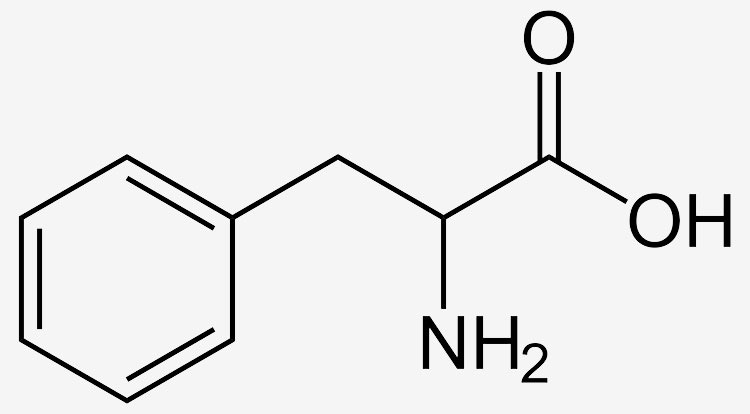
\includegraphics[scale=0.2]{fe}
\end{figure}
\begin{figure}[H]
\centering
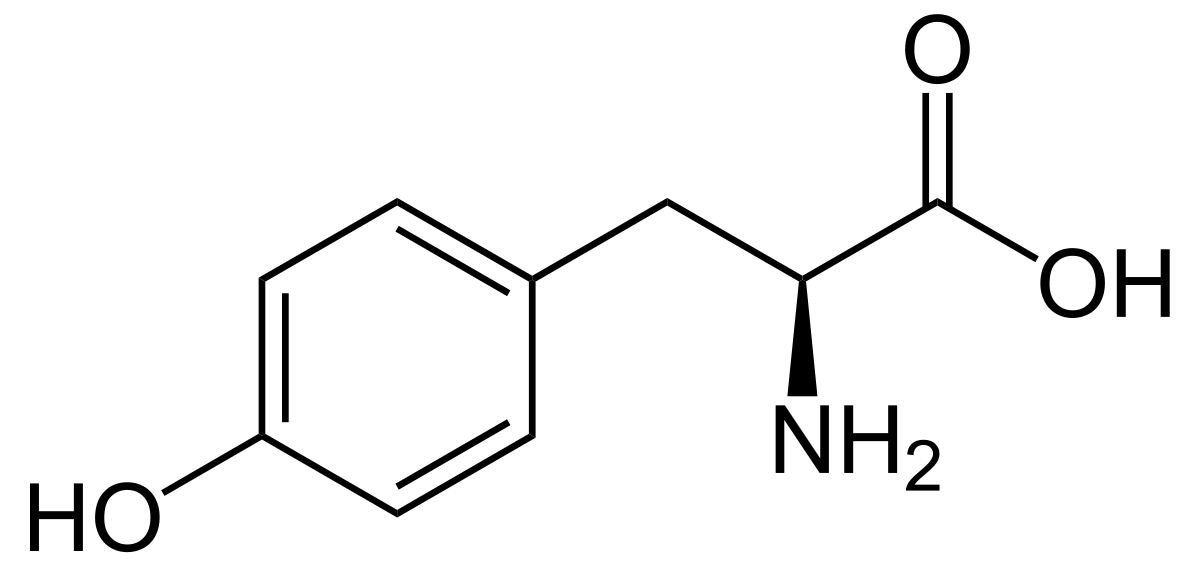
\includegraphics[scale=0.25]{ti}
\caption{Comparación estructural provocada por la mutación de PHE a TYR}
\end{figure}

Hemos seleccionado tres tirosinas al azar de la proteína para estudiar como se comportaban sus vectores para obtener el módulo promedio $\left\| m \right\|$. Con ellos hemos determinado el módulo del vector. Esto nos ha permitido posteriormente con nuestra fenilalanina de interés calcular el vector unitario $\overrightarrow{U}$, y finalmente obtener el vector $\overrightarrow{v}$ de interés, lo que nos permite conocer las coordenadas teóricas del grupo OH.
\newline

\begin{equation}
\left\| m \right\|=\overrightarrow{O}- \overrightarrow{CZ}
\end{equation}
\begin{equation}
\overrightarrow{D}=\overrightarrow{CZ}- \overrightarrow{CB}
\end{equation}
\begin{equation}
\overrightarrow{U}=\frac{D}{\left\| D \right\|}
\end{equation}

Con lo que finalmente obtenemos:
\begin{equation}
\overrightarrow{V}=\overrightarrow{U} * \left\| m \right\|
\end{equation}

Finalmente, tomamos el $\overrightarrow{CZ}$ de nuestro residuo, sumándole el vector $\overrightarrow{V}$ a mutar y añadimos una línea ATOM nueva con las coordenadas obtenidas, siguiendo el mismo sentido que el esqueleto del anillo aromático.

\begin{figure}[H]
\centering
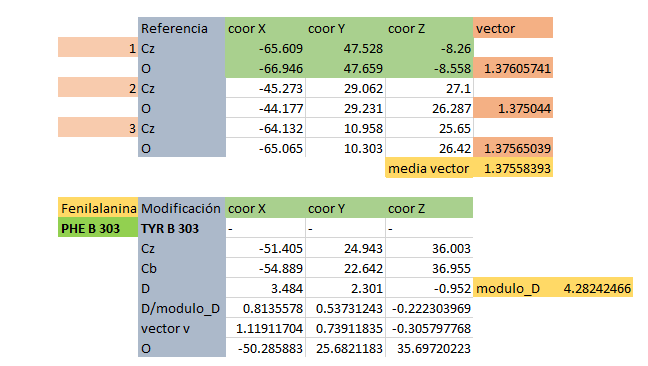
\includegraphics[scale=0.7]{Screenshot_44}
\caption{Matriz de cálculos realizados en el software Excel}
\end{figure}


\begin{figure}[H]
\centering
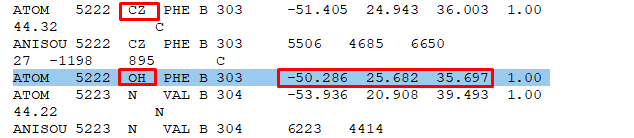
\includegraphics[scale=0.7]{Screenshot_45}
\caption{Línea ATOM creada}
\end{figure}

La mutación se ha producido en el dominio NendoU, responsable de la actividad catalítica, muy cerca además del centro activo, por lo que la carga introducida podría modificar la estructura del mismo y por ende, modificar su acción. Adicionalmente, la mutación afecta a un residuo que se encuentra en una zona hidrofóbica en el interior de la proteína, por lo que podría crear una mayor repulsión de cargas.


\begin{figure}[H]
\centering
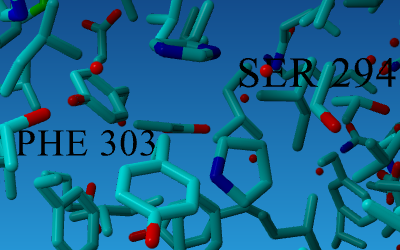
\includegraphics[scale=0.9]{mut}
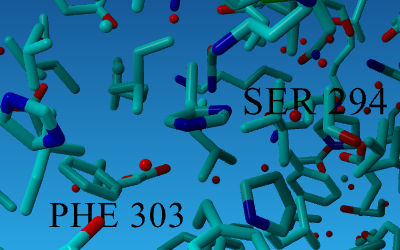
\includegraphics[scale=0.9]{nomut}
\caption{Visualización de la proteína mutada (arriba) y la proteína silvestre(abajo)}
\end{figure}
 

\subsubsection{Enlaces disulfuro}
En esta actividad hemos realizado un programa que recorre los átomos de la proteína buscando los átomos sulfuro cisteínas con ID ``SG'', es decir, los que pueden dar lugar a la formación de puentes disulfuro.
\newline

En este ejercicio la distancia entre los átomos de sulfuro es esencial, pues de esta depende que se puedan crear este tipo de puentes, ya que solo a determinadas distancias se dan las energías correctas para su estabilización. Además, mientras unas proteínas pueden tener una gran cantidad de este tipo de enlaces, otras pueden carecer completamente de ellos.
\newline

Por ello, realizamos previamente al estudio de nuestra proteína un screening con otras que utilizamos de base para encontrar la distancia en Angstrom adecuada para que se den los puentes disulfuro.
\newline

Por ejemplo, 1HAI y 1BHS no contiene ninguno, mientras que otras como 2ZUP contiene apenas 2 y 2QWQ únicamente 1, y otras como 1AFD tiene hasta 6 enlaces. Del muestreo realizado deducimos que la distancia correcta para el enlace disulfuro se encuentra aproximadamente en 2.05 Angstrom, si bien podemos dar por válidas distancian un poco mayores para asegurarnos de no perder ningún puente disulfuro.

\begin{figure}[H]
\centering
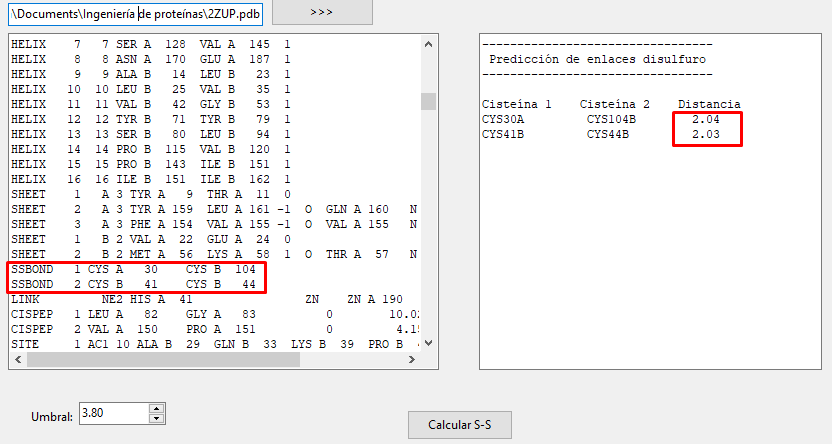
\includegraphics[scale=0.5]{Screenshot_38}
\end{figure}
\begin{figure}[H]
\centering
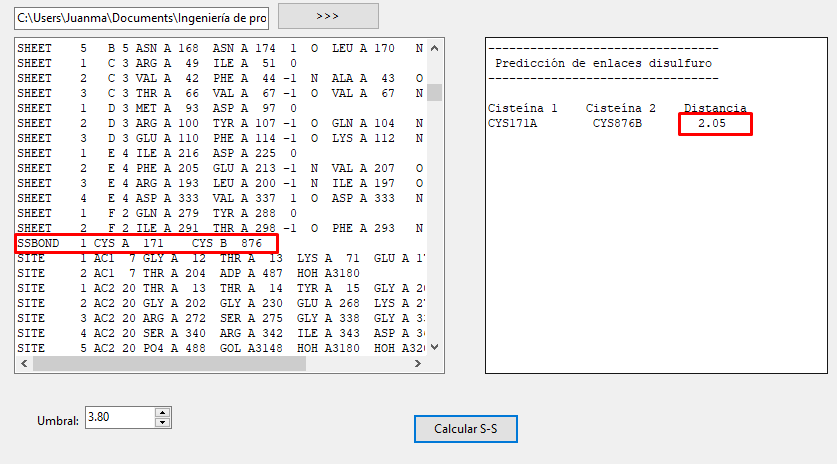
\includegraphics[scale=0.5]{Screenshot_39}
\end{figure}
\begin{figure}[H]
\centering
\includegraphics[scale=0.5]{Screenshot_40}
\caption{Imágenes tomadas de la aplicación ``Enlaces SS'' para tomar referencias de cara al estudio de los enlaces disulfuro en nuestra proteína de interés Nsp15}
\end{figure}

Para asegurarnos que nuestra predicción era correcta, comprobamos que no existía ningún apartado para enlaces disulfuro en el archivo PDB de la proteína, y además en YASARA tampoco encontramos ninguno.

\subsubsection{Anfipatía-hidrofobicidad}
La hidrofobicidad es una fuerza dominante en la formación de la estructura tridimensional plegada de la proteína. Básicamente se refiere a la fuerza que controla que las regiones apolares no estén expuestas al solvente polar, impidiendo la formación de clatratos, estructuras muy ordenadas y desfavorables a nivel energético. Por ende, se formarán interacciones entre moléculas hidrofóbicas, lo que redunda en una disminución neta de la energía del sistema. Por tanto, hablamos de una fuerza esencialmente entrópica. 

\begin{equation}
\Delta{G}=\Delta{H} - T\Delta{S}
\end{equation}
\newline

Teniendo en cuenta que todos los residuos comparten su esqueleto covalente, la hidrofobicidad vendrá determinada por el carácter hidrofóbico de las cadenas laterales. No obstante, es muy complicado obtener un valor directo de la hidrofobicidad de cada residuo, pues se ve influenciado por el ambiente en el que se encuentra.
\newline

Por ello, existen diversas escalas hidrofóbicas, donde podemos destacar alguna como es el caso de la de ``doolittle''. Habrá que cargar esta escala en nuestra aplicación para poder llevar a cabo el análisis correspondiente.
\newline

Desgraciadamente, obtener el valor de hidrofobicidad correspondiente a cada residuo es una tarea muy compleja, por lo que la estrategia a seguir será la de asignar a un residuo el valor promedio de la hidrofobicidad obtenida de una ventana de residuos contiguos a través del ``moving average''. De esta manera podremos reducir el ruido y mejorar la fiabilidad de nuestros datos. Esto ha sido denominado ``método de suavizado de Savinski-Golay''.
\newline


Otro factor importante que mediremos en este programa es la denominada anfipatía, que se refiere a la hidrofobicidad medida en la distribución de la estructura secundaria de la proteína. Utilizamos dos métodos para el estudio de dicha anfipatía:

\begin{enumerate}
\item Eisenberg. Este método se basa en en el estudio del momento hidrofóbico midiendo magnitudes físicas, estableciéndolo la hidrofobicidad total como una suma de vectores 

\begin{equation}
\mu_H =\sqrt{(\sum H_n\sin(\delta n))^2 +(\sum H_n \cos(\delta n))^2}
\end{equation}

\item Stroud. Este método se basa en el uso de magnitudes matemáticas (``Fourier Power Spectrum''). De la transformada de Fourier se obtiene la amplitud repecto a la frecuencia del  momento armónico representado. 

\begin{equation}
I(k, v) =(\sum_{j=k-n}^{k+n} (h_j- \bar{h}(k))\sin(jv))^2 + (\sum_{j=k-n}^{k+n} (h_j- \bar{h}(k))cos(jv))^2
\end{equation}

\end{enumerate}

En lo referido a nuestro programa, la estrategia seguida será la siguiente.
\newline

Necesitaremos 3 inputs: la proteína elegida, la semiventana y la escala. Además, podremos seleccionar los residuos en los que mediremos la hidrofobicidad y anfipatía. Cargaremos los datos obtenidos a partir de las ecuaciones correspondientes en una estructura TTablaDatos, y con esta podremos representar los perfiles hidrofóbicos mediante un plot.

\begin{figure}[H]
\centering
\includegraphics[scale=0.6]{Screenshot_46}
\caption{Imágenes correspondientes a los perfiles de hidrofobicidad, anfipatía por Eisenberg y anfipatía por Stroud}
\end{figure}

Como podemos observar los datos obtenidos en las gráficas son similares, lo que realza nuestra confianza en el programa. Podemos inferir que los puntos altos de las gráficas de anfipatía se corresponden con hélices $\alpha$, pues la anfipatía se define como la lateralidad de la hidrofobicidad, lo que sucede en cada giro de la hélice. Por su parte los ``llanos'' de la gráfica se corresponden con láminas $\beta$, que tienen una menor anfipatía por su disposición. No obstante, esto puede llevarnos a falsas interpretaciones, y es muy importante optimizar en cada caso la semiventana utilizada.
\newpage
\bibliography{Base_datos_covid}
\end{document}